\documentclass[12pt]{article}
\usepackage{babel}
\usepackage[utf8x]{inputenc}
\usepackage[T1]{fontenc}
\usepackage[colorinlistoftodos]{todonotes}
\usepackage{listings}
\usepackage{amssymb}
\usepackage{amsmath}
\usepackage{amsthm}
\usepackage{appendix}
\usepackage{multicol}
\usepackage{stmaryrd}
\usepackage{algorithm, algorithmic}

\theoremstyle{plain}
\newtheorem{thm}{Théorème}[section]
\newtheorem{lemme}[thm]{Lemme}
\newtheorem{propo}[thm]{Proposition}

\theoremstyle{definition}
\newtheorem{remarque}[thm]{Remarque}
\newtheorem{defi}[thm]{Définition}
\newtheorem{nota}[thm]{Notation}


\renewcommand{\a}{\alpha}
\newcommand{\HRule}{\rule{\linewidth}{0.5mm}} 
\newcommand{\F}{\mathbb{F}} 
\newcommand{\A}{\mathcal{A}} 
\newcommand{\e}{\mathbf{e}}  
\newcommand{\s}{\mathbf{s}} 
\newcommand{\K}{\mathbb{K}} 
\newcommand{\J}{\mathcal{J}} 
\newcommand{\D}{\mathcal{D}} 

% traduction des mots pour les algos
\floatname{algorithm}{Algorithme}
\renewcommand{\algorithmicrequire}{\textbf{Entrées:}}
\renewcommand{\algorithmicensure}{\textbf{Sortie:}}
\renewcommand{\algorithmicrepeat}{\textbf{Faire}}
\renewcommand{\algorithmicuntil}{\textbf{Tant que}}
\renewcommand{\algorithmicreturn}{\textbf{Retourne}}

\renewcommand{\contentsname}{Sommaire}

\title{Projet - Wave}
\author{Lansade Suzanne}
\author{Palandjian Eva}

\begin{document}

\begin{titlepage}

\center

\textsc{\LARGE Université de Bordeaux}\\[2.0cm]
\textsc{\Large Master 2 : Cryptologie et Sécurité Informatique}\\[0.5cm] 
\textsc{\large Projet de fin d'études}\\[1.2cm] 

\HRule \\[0.4cm]
{ \huge \bfseries Wave - Un procédé de signature \\ à base de codes correcteurs}\\[0.3cm] 
\HRule \\[1.3cm]


\begin{minipage}{0.4\textwidth}
\begin{flushleft} \large
Suzanne \textsc{Lansade}\\
Eva \textsc{Palandjian}\\
\end{flushleft}
\end{minipage}
~
\begin{minipage}{0.4\textwidth}
\begin{flushright} \large
\emph{Encadrant:} \\
Gilles \textsc{Zemor}
\end{flushright}
\end{minipage}\\[2cm]

\begin{large}
Février, 2020
\end{large}

\vspace{0.5in}


\includegraphics [scale=0.2]{include/Universite_Bordeaux.jpg}

\end{titlepage}

\newpage
\tableofcontents
\newpage

\section*{Introduction}
\addcontentsline{toc}{section}{\protect\numberline{}Introduction}
Dans le milieu des années 70, la cryptograhie à clé publique fut marquée par l'arrivée du chiffrement RSA ainsi que du protocole d'échange de clés Diffie-Hellman. De nos jours, ces deux méthodes sont les plus utilisées en pratique. Le chriffrement RSA repose sur le problème de la factorisation, tandis que le protocole DH repose sur le problème de la résolution du logarithme discret. La cryptographie à clef publique repose donc principalement sur ces deux problèmes, tous les deux des instances du problème dit du sous-groupe caché dans un groupe abélien. Il n’existe pas à ce jour d’attaque classique contre ce problème. \\ 

\noindent En revanche, il existe des attaques utilisant des algorithmes quantiques. \\
Dans le contexte de l'éventualité de l'arrivée dans les décénies à venir de l'ordinateur quantique, le National Institute of Standard Technology (NIST) lança en 2017 un appel pour la standardisation de systèmes à clef publique, afin de trouver des alternatives à RSA et DH.
Le papier sur lequel nous avons travaillé propose un système de signature à base de code correcteurs. Les codes correcteurs, que l'on sait déjà utiliser depuis les années 70 pour le chiffrement (ex: crypto-système de McEliece) présentent une alternative quantiquement sûr puisqu'ils reposent sur le problème du décodage, un problème NP-complet. En revanche, les recherches pour utiliser des codes dans des systèmes de signatures sont peu concluantes, en témoigne le tableau des soumissions au NIST pour le second tour. \\

\begin{figure}[h]
\label{nist 2}
\begin{center}
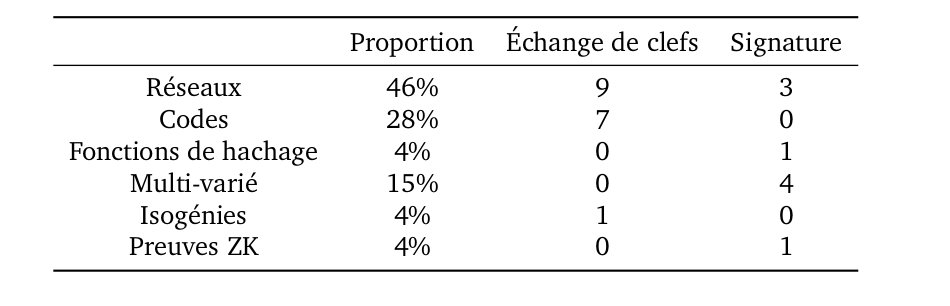
\includegraphics [scale=0.4]{include/nist_second_tour.png}
\end{center}
\caption{\small Comparaison des soumissions au NIST du second tour.}
\end{figure}
\noindent Alors pourquoi est-il si compliqué de faire des signatures avec des codes correcteurs ? \\
Premièrement, il est difficile de tomber dans l'ensemble des syndromes facilement décodables, dans le sens où il est difficile de créer une fonction de hachage qui envoie le message $m$ dans l'ensemble des syndromes possibles. En effet, pour un décodage au sens stricte, il faudrait un syndrome $s$ associé à un unique mot $c$ du code, le plus proche de $m$.\\
Cela ne pose pas de problème lorsqu'on chiffre, puisque notre chiffré sera justement le syndrome. Il suffit donc de choisir un vecteur erreur en conséquance, et de le transformer en le syndrome associé. Le déchiffrement consistera alors à retrouver le vecteur erreur à partir du syndrome. \\
En revanche, pour la signature, il faudra trouver un moyen de transformer notre message en un syndrome qui sera dans l'ensemble des syndromes associés à un vecteur erreur de poids minimal. \\
Tous les systèmes de signatures basés sur des codes sont pour l'instant soit cassés, soit inutilisables dans la pratique.\\

\noindent La solution de Wave est d'enlever la restriction au mot le plus proche. On cherche maintenant une famille de codes permettant de trouver, pour un mot quelconque, un des mots de code à distance $\omega$. En particulier, la distance de décodage $\omega$ est très grande, ce qui assure typiquement de l’existence d’un mot de code à cette distance. Ainsi, l'ensemble des syndromes utilisables est l'ensemble de tous les syndromes.\\
Nous expliquerons dans ce rapport comment fonctionne le système de signature Wave. Nous montrerons ensuite comment s'assurer qu'il ne fait pas fuiter d'information grâce à une uniformisation des sorties, puis nous démontrerons qu'il est sûr pour la sécurité EUF-CMA.

\section{Le schéma de signature Wave}
Nous allons détailler dans cette section le schéma de signature Wave. C'est un schéma de type hache et signe à base de codes correcteurs. Pour des raisons de clarté nous oublierons dans un premier temps la problématique du hachage. Nous la réintroduirons en fin de rapport afin de proposer une preuve formelle de la sécurité du schéma, où la fonction de hachage est alors nécessaire. Pour l'instant, nous considérerons que l'entrée de l'algorithme de signature est déjà un syndrome.\\
Le schéma de signature Wave s'appuie sur une famille de codes appelés des codes $(U,U+V)$-généralisés. La structure de ces codes nous permettra de proposer un algorithme de décodage $\mathcal{D}$ utilisant une trappe $T$ et donnant un avantage par rapport à un algorithme de décodage générique. Ce système s'appuie aussi sur la notion de fonctions GPVM, que nous détaillerons. \\

\subsection{La famille de codes (U,U+V)-généralisés}
Pour définir la famille de code utilisée dans le schéma de signature Wave, on partira de deux codes de longueur $n/2$ aléatoires de dimensions respectives $k_U$ et $k_V$. Nous avons la définition suivante :

\begin{defi}\label{UV} (Code $(U,U+V)$) Un code $(U,U+V)$ est un code de longueur $n$ et de dimension $k=k_U+k_V$ et tel que :
\begin{center}
$(U,U+V) = \{(u,u+v)$ tel que $u \in U$ et $v \in V \}$
\end{center}
\end{defi}


\noindent En revanche, pour le système de signature Wave, nous n'utiliserons pas cette définition. En effet, nous allons voir que l'on peut facilement tirer des informations sur la structure de ces codes.\\


\begin{defi} Le  $hull$ d'un code $\mathcal{C}$ est défini comme $hull(\mathcal{C}) := \mathcal{C} \cap \mathcal{C}^{\bot}$
\end{defi}

\begin{propo}\label{dim_hull}
Soit $\mathcal{C}$ un code aléatoire binaire de longueur $n$ et de dimension $k$, alors on s'attend à avoir $dim(hull(\mathcal{C}))\sim\mathcal{O}(1)$. De plus : $$ \mathbb{P}\big(dim(hull(\mathcal{C})\big) \leq t) \ \geq\ 1 - \mathcal{O}(2^{-t}) $$
\end{propo}

\begin{propo}\label{dim_hull_UV}
Soit $UV$ un code $(U,U+V)$-binaire de longueur $n$ tel que $k_U > k_V$, alors nous avons avec probabilité $1-\mathcal{O}(2^{k_U-k_V})$
$$ dim(hull(UV)) = k_U - k_V $$
\end{propo}



\begin{proof}[Preuve]
Montrons que nous avons $dim(hull(U,U+V)) = k_U - k_V$ avec probabilité $1-\mathcal{O}(2^{k_U-k_V})$.
Par définition du $hull$, nous avons :
\begin{equation*}
\begin{split}
hull(U,U+V) &= (U,U+V) \cap (U,U+V)^{\bot } \\
&= (U,U+V) \cap (V^{\bot}+U^{\bot}, V^{\bot}) \\
\end{split}
\end{equation*} 
Ainsi $\forall u\in U$ et $\forall v\in V$ tels que $(u,u+v)\in hull(U,U+V)$, il existe $u^{\bot}\in U^{\bot}$ et $v^{\bot}\in V^{\bot}$ tels que

\begin{equation*}
\left\{
\begin{aligned}
&u = v^{\bot} + u^{\bot}\\
&u + v = v^{\bot}\\
\end{aligned}
\right.
\iff
\left\{
\begin{aligned}
&v = u^{\bot}\\
&u + v = v^{\bot}\\
\end{aligned}
\right.
\end{equation*}
Donc $v\in V\cap U^{\bot}$.
De plus, nous avons $$\dim(V) + \dim(U^{\bot}) = \frac{n}{2} +k_V - k_U < \frac{n}{2}$$
Alors, avec probabilité $1-0(2^{k_V-k_U})$ sur le choix des codes, nous aurons $V \cap U^{\bot} = {0}$ et $v=u^{\bot} = 0$. Ainsi, les vecteurs de $hull(U,U+V)$ seront de la forme $(x,x)$ où $x \in U \cap V^{\bot}$ avec probabilité  $1-0(2^{k_V-k_U})$ .
De même on a,
$$\dim(U) + \dim(V^{\bot}) = \frac{n}{2} +k_U - k_V < \frac{n}{2}$$

\noindent Alors avec probabilité $1-0(2^{k_V-k_U})$, on aura 
$$\dim(\text{hull}((U,U+V))) = \dim(U\cap V^{\bot}) = k_U-k_V $$
ce qui conclue la preuve.
\end{proof}

\noindent Ainsi nous ne pouvons pas utiliser les codes $(U,U+V)$ binaires où $\dim(U) > \dim(V)$ puisque nous pouvons facilement les distinguer de codes aléatoires.
En effet, il suffit de calculer la dimension de  leur $hull$ puis de le comparer au résultat de la proposition \ref{dim_hull}.
Pour résoudre ce problème, nous poserons $q=3$ pour toute la suite du rapport, nous pouvons alors travailler avec $\dim(U) > \dim(V)$. \\
Dans la pratique, les sorties de l'algorithme de signature seraient permutées afin de cacher la structure du code. Ainsi, comme vu dans la preuve, le fait que des éléments de la forme $(x,x)$ apparaissent avec bonne probabilité pose un problème puisque cela révèle des informations sur cette permutation, partie intégrante du secret. \\
Pour pallier à cela nous utiliserons une nouvelle famille de codes, les codes $(U,U+V)$-généralisés :\\
\newpage
\begin{defi} \label{UV-normalise} (codes $(U,U+V)$-généralisés) Soient $n$ un entier pair et $a$,$b$,$c$,$d$ quatres vecteurs de $\F_q^{n/2}$ tels que pour tout $i \in \llbracket 1,n/2\rrbracket$ :
\begin{equation}\label{ac}
a_ic_i \neq 0 
\end{equation}
\begin{equation}\label{ad-bc}
a_id_i - b_ic_i \neq 0 
\end{equation}

\noindent Soient U et V deux codes définis comme précédemment. Le code $(U,U+V)$-généralisé correspond à l'ensemble :
\begin{center}
$\{(a.u + b.v, c.u + d.v)$ tel que $u \in U$ et $v \in V \}$
\end{center}
où $x.y$ est le produit coordonnée par coordonnée des $x_i$ et $y_i$.\\
\end{defi}


\noindent Les conditions sur les vecteurs $a$, $b$, $c$, $d$ permettent de garantir que :
\begin{itemize}
\item[-] toutes les coordonnées de $u \in U$ apparaîtront deux fois, ce qui sera nécessaire pour utiliser la structure du code dans notre algorithme de décodage (par l'équation \eqref{ac}).
\item[-] la dimension du code $(U,U+V)$-généralisé sera la somme des dimensions des codes $U$ et $V$ (par l'équation \eqref{ad-bc}).
\end{itemize}

\noindent Sans perte de généralité, nous posons pour toute la suite les vecteurs $a$,$b$,$c$,$d$ tels que $a_id_i - b_ic_i = 1 \text{ pour tout } i \in \llbracket 1,n/2\rrbracket$ Nous pourrons toujours nous ramener au cas général. \\

\begin{propo} Soient $U$, $V$, $a$, $b$, $c$ et $d$ définis comme précédemment. Soit $UV$ le code $(U,U+V)$-généralisé associé. Alors
$$ k = \dim\; (UV) = k_U + k_V.$$
De plus soient:
\begin{itemize}
\item$G_U \in \F_q^{k_U \times n/2}$ (respectivement $G_V \in \F_q^{k_V \times n/2}$)
\item$H_U \in \F_q^{(n/2-k_U) \times n/2}$ (respectivement $H_V \in \F_q^{(n/2-k_V) \times n/2}$) 
\end{itemize}  les matrices génératrices et de parité des codes $U$ et $V$. \\
Soient $A$, $B$, $C$, $D$ de $\F_q^{n \times n}$ les matrices diagonales de diagonales respectives les vecteurs $a$, $b$, $c$ et $d$.  \\

\noindent Alors la matrice de $\F_q^{(k_U + k_V) \times n}$: 

\vspace{0.1in}

$$
G := 
\begin{pmatrix}
\begin{array}{c|c}
G_UA & G_UC \\
 \hline 
G_VB & G_VD \\
\end{array} \\
\end{pmatrix}
$$

\noindent et la matrice $\F_q^{(n - k_U - k_V) \times n}$:

\vspace{0.1in}
$$ 
H :=
\begin{pmatrix}
\begin{array}{c|c}
H_UD & -H_UB \\
 \hline 
-H_VC & H_VA \\
\end{array} \\
\end{pmatrix}
$$
\vspace{0.1in}

\noindent sont les matrices génératrice et de parité du code $UV$. 
\end{propo}

\begin{proof}[Preuve]
Remarquons d'abord que G engendre bien le code $UV$. Remarquons aussi que 

$$
G = 
\begin{pmatrix}
\begin{array}{c|c}
G_UA & G_UC \\
 \hline 
G_VB & G_VD \\
\end{array} \\
\end{pmatrix}
= 
\begin{pmatrix}
\begin{array}{c|c}
G_U & 0 \\
 \hline 
0 & G_V \\
\end{array} \\
\end{pmatrix} 
\begin{pmatrix}
\begin{array}{c|c}
A & C \\
 \hline 
B & D \\
\end{array} \\
\end{pmatrix}
$$

\noindent Par définition des matrices $G_V$ et $G_U$, la matrice $ 
\begin{pmatrix}
\begin{array}{c|c}
G_U & 0 \\
 \hline 
0 & G_V \\
\end{array} \\
\end{pmatrix} $ est de rang $k_U + k_V$. De plus les matrices $A$, $B$, $C$, $D$ étant diagonales, le déterminant de la matrice $\begin{pmatrix}
\begin{array}{c|c}
A & C \\
 \hline 
B & D \\
\end{array} \\
\end{pmatrix}$
est le produit des $(a_id_i - b_ic_i)$ pour $i \in \llbracket 1, n/2\rrbracket$, et donc non-nul par définition des vecteurs $a,b,c,d$. On a donc bien $k = k_U + k_V$. \\
On remarque aussi que $GH^T = 0$ et que $H$ est de rang plein par le même raisonnement que précédemment, ce qui conclut la preuve.
\end{proof}



\subsection{Le principe de signature}

Notre schéma de signature utilisera donc les codes $(U,U+V)$-généralisés et la fonction syndrome comme fonction à sens unique (sous l'hypothèse de la difficulté de résoudre le problème du décodage). \\

\noindent Nous allons définir la notion de fonctions GPV en moyenne (GPVM). Pour cela, introduisons d'abord la notion de distance statistique.

\begin{defi}
Soient $X$ et $Y$ deux variables aléatoires à valeurs dans le même espace $\epsilon$. 
Soient $\mathcal{D}_X$ et $\mathcal{D}_Y$ leurs distributions respectives. On définit la distance statistique entre ces deux distributions comme :
$$ \rho(\mathcal{D}_X,\mathcal{D}_Y) := \frac{1}{2} \sum_{x \in \epsilon} |\mathcal{D}_X(x) - \mathcal{D}_Y(x)|.$$
\end{defi}

\begin{defi} (Fonctions GPVM). On appelle fonction GPV en moyenne une paire d'algorithmes (\verb|Trapdoor|,\verb|InvertAlg|) ainsi qu'un triplet de fonctions ($n(\lambda),k(\lambda),\omega(\lambda)$) en fonction d'un paramètre de sécurité $\lambda$, tels que :
\begin{itemize}
\item \verb|Trapdoor| est un algorithme probabiliste et polynomial en $1^\lambda$ et renvoyant le couple $(H,T)$ où $H \in \F_q^{(n-k) \times n}$ de rang $n-k$ et $T$ est la trappe associée.
\item \verb|InvertAlg| est un algorithme probabiliste et polynomial prenant en entrée la trappe $T$ et un syndrôme $s \in \F_q^{n-k}$, et renvoyant $e \in \F_q^{n}$ de poids $\omega$ tel que $eH^T = s$.
\end{itemize}
De plus, pour \textit{presque toute} matrice $H$ renvoyée par \verb|Trapdoor|, la fonction est :
\begin{enumerate}
\item bien distribuée : 
$$\rho(eH^T,s) \in \text{negl}(\lambda)$$ où $e$ est pris uniformément dans l'ensemble des mots de poids $\omega$ et de longueur $n$ et $s$ est pris uniformément dans $\F_q^{n-k}$. 
\item sans fuite d'information \textit{en moyenne} : 
$$ \rho(\verb|InvertAlg|(s,T),e) \in \text{negl}(\lambda)$$ où $e$ est pris uniformément dans l'ensemble des mots de poids $\omega$ et de longueur $n$ et $s$ est pris uniformément dans $\F_q^{n-k}$. 
\item \`A sens unique sans la trappe : 
$$\mathbb{P}(\mathcal{A}(H,s) = e \;| \;eH^T = s) \in \text{negl}(\lambda)$$
pour tout algorithme probabiliste polynomial $\mathcal{A}$.
\end{enumerate}
C'est une définition relaxée des fonctions GPV.
\end{defi}

\noindent Nous générons notre paire de clés publique et privée comme :
$$ (pk, sk) = (H,T) \leftarrow \verb|Trapdoor|(\lambda)$$
Plus précisément, dans notre cas, nous aurons donc pour clé publique la matrice de parité du code $(U,U+V)$-généralisé, notée $H$, et pour clé privée, les matrices de parité des codes $U$ et $V$, respectivement notées $H_U$ et $H_V$.\\
Notre algorithme $\verb|InvertAlg|$ sera un algorithme utilisant la structure des codes  $(U,U+V)$-généralisés afin d'inverser la fonction syndrome avec un avantage par rapport à un algorithme de décodage générique. \\
Le troisième point de la définition est bien vérifié, puisqu'il découle directement de la difficulté d'inverser la fonction syndrome. De plus, la fonction syndrome est en effet bien distribuée, même si nous ne le montrerons pas dans ce rapport. Enfin, le caractère sans fuite d'information de notre système sera discuté dans la deuxième partie du rapport. \\
Nous pouvons maintenant définir notre système de signature.
\begin{multicols}{2}
\begin{flushleft}
$\verb|Sign|^{sk}(s)$:\\
	$\quad$ e $\leftarrow$  \verb|InvertAlg|(s,T) \\
	$\quad$ \verb|renvoie| e
\end{flushleft}
\begin{flushleft}
$\verb|Verify|^{pk}(s,e')$: \\
	$\quad \verb| Si | e'H^T = s \verb| et | |e'| = \omega $ \\
	$\quad \quad$ \verb|renvoie 1| \\
	$\quad$ \verb|renvoie 0|
\end{flushleft}
\end{multicols}


\subsection{Le décodage avec trappe}

En partant de l'hypothèse que la matrice de parité $\mathbf{H}$ du code $(U,U+V)$-généralisé ressemble à une matrice aléatoire, la difficulté de créer une fausse signature sans connaître la trappe $T$ est exactement celle de résoudre le problème du décodage d'un code aléatoire, que l'on sait difficile. Nous allons expliciter dans cette section l'algorithme d'inversion de la fonction syndrome connaissant la trappe, et discuter de sa difficulté en fonction du poids $\omega$ de $\e$. \\

\noindent Notons $\mathcal{S}_{\omega,n}$ l'ensemble des mots de poids $\omega$ et de longueur $n$. On notera dans la suite $\mathcal{S}_{\omega}$ s'il n'y a pas d’ambiguïté sur la longueur. On rappelle que l'algorithme \verb|InvertAlg| cherche à inverser la fonction syndrome : 
$$\begin{array}{ccccc}
f_{\omega,\mathbf{H}} & : & \mathcal{S}_{\omega,n} & \to & \F_q^{n-k} \\
 & & \mathbf{e} & \mapsto & \mathbf{eH^T} \\
\end{array}$$

\noindent On rappelle aussi que la fonction $f_{\omega,\mathbf{H}}$ avec $\mathbf{H} \in \F_q^{(n-k)\times n}$ s'inverse génériquement si $\omega \in \llbracket\omega_{easy}^-,\omega_{easy}^+\rrbracket$, où :
$$ \omega_{easy}^- := \frac{q-1}{q}(n-k) \qquad \text{ et }\qquad  \omega_{easy}^+ := k + \frac{q-1}{q}(n-k).$$




\noindent De plus la fonction $f_{\omega,\mathbf{H}}$ admet un inverse pour toute entrée $s \in \F_q^{n-k}$ si $\omega \in \llbracket\omega^-,\omega^+\rrbracket$, où :
$$\omega^- := \min\left\{\omega\in \llbracket0,n\rrbracket , \dbinom{\omega}{n}(q-1)^{\omega} \geq q^{n-k}\right\} $$
$$\omega^+ := \max\left\{\omega\in \llbracket0,n\rrbracket , \dbinom{\omega}{n}(q-1)^{\omega} \geq q^{n-k}\right\}$$


\noindent Nous voulons donc un moyen d'inverser la fonction syndrome pour $\omega \in \llbracket\omega_{UV}^-,\omega_{UV}^+\rrbracket$ avec $\omega_{UV}^-$ et $\omega_{UV}^+$ tels que :

$$\llbracket\omega_{easy}^-,\omega_{easy}^+\rrbracket \subsetneq \llbracket\omega_{UV}^-,\omega_{UV}^+\rrbracket \subset  \llbracket\omega^-,\omega^+\rrbracket$$


\noindent Afin d'expliciter le décodage, introduisons la fonction :

$$\begin{array}{ccccc}
\varphi_{\mathbf{a},\mathbf{b},\mathbf{c},\mathbf{d}} & : & \F_q^{n/2} \times  \F_q^{n/2} & \to & \F_q^{n/2} \times  \F_q^{n/2} \\
 & & (\mathbf{x} , \mathbf{y}) & \mapsto &  (a.\mathbf{x} + b.\mathbf{y}, c.\mathbf{x} + d.\mathbf{y}) \\
\end{array}$$

\noindent Si cette fonction respecte les conditions sur les vecteurs $a,b,c,d$ définies dans la définition \ref{UV-normalise}, on dit qu'elle est UV-normalisée. Dans ce cas on peut vérifier qu'elle est bijective d'inverse :

\vspace{0.2in}
$$\begin{array}{ccccc}
\varphi^{-1}_{a,b,c,d} & : & \F_q^{n/2} \times  \F_q^{n/2} & \to & \F_q^{n/2} \times  \F_q^{n/2} \\
 & & (\mathbf{x} , \mathbf{y}) & \mapsto &  (d.\mathbf{x} - b.\mathbf{y}, -c.\mathbf{x} + a.\mathbf{y}) \\
\end{array}$$

\vspace{0.2in}

\noindent Ainsi, pour chaque vecteur $\mathbf{e}$ de $\F_q^n$, on peut associer deux vecteurs $\mathbf{e_U}$ et $\mathbf{e_V}$ de $\F_q^{n/2}$ tels que 
$$ (\mathbf{e_U},\mathbf{e_V}) = \varphi^{-1}_{a,b,c,d}(\mathbf{e}).$$

\begin{propo} Inverser $f_{\omega,\mathbf{H}}$ pour un certain $\mathbf{s} \in F_q^{n-k}$ est équivalent à trouver $\mathbf{e} \in \F_q^n$ tel que:
$$ \mathbf{e}_U\mathbf{H}_U^T = \mathbf{s}^U \qquad \text{et} \qquad \mathbf{e}_V\mathbf{H}_V^T = \mathbf{s}^V $$

\vspace{0.1in}
où $\mathbf{s} = (\mathbf{s}^U, \mathbf{s}^V)$ avec $\mathbf{s}^U \in \F_q^{n/2-k_U}$ et $\mathbf{s}^V \in \F_q^{n/2-k_V}$.
\end{propo}

\vspace{0.2in}
\begin{proof}[Preuve]
Nous voulons montrer que le syndrome de $\e$ vaut $(\e_U\mathbf{H}_U^T,\e_V\mathbf{H}_V^T)$.
Remarquons d'abord que nous avons
\begin{equation*}
\begin{split}
\e &= \varphi(\e_U,\e_V)\\
&= (\mathbf{a}.\e_U + \mathbf{b}.\e_V,\ \mathbf{c}.\e_U + \mathbf{d}.\e_V)\\
&= (\e_U A + \e_V B,\ \e_U C + \e_V D)\\
\end{split}
\end{equation*}

\noindent avec $A$, $B$, $C$, $D$ les matrices diagonales définie auparavant.\\
De plus, notons que

\vspace{0.1in}
$$ 
H^T :=
\begin{pmatrix}
\begin{array}{c|c}
D^TH_U^T & -C^TH_V^T \\
 \hline 
-B^TH_U^T & A^TH_V^T \\
\end{array} \\
\end{pmatrix}
$$
\vspace{0.1in}

\noindent Nous avons $\e\mathbf{H}^T = \s = (\s^U,\ \s^V)$. Ainsi, en calculant le syndrome de $\e$ à l'aide des expressions précédentes, nous obtenons :

\begin{equation*}
\begin{aligned}
&\left\{
\begin{split}
(\e_UA+\e_VB)D^T\mathbf{H}_U^T - (\e_UC+\e_VD)B^T\mathbf{H}_U^T &= \s^U \\ 
-(\e_UA+\e_VB)C^T\mathbf{H}_V^T + (\e_UC+\e_VD)A^T\mathbf{H}_V^T &= \s^V \\
\end{split}
\right.\\
\\
\iff
&\left\{
\begin{split}
\e_U(AD^T - CB^T)\mathbf{H}_U^T + \e_V(BD^T-CB^T)\mathbf{H}_U^T &= \s^U \\ 
\e_U(CA^T - AC^T)\mathbf{H}_V^T + \e_V(DA^T-BC^T)\mathbf{H}_V^T &= \s^V \\ 
\end{split}
\right.
\end{aligned}
\end{equation*}\

\noindent Comme $A$, $B$, $C$ et $D$ sont des matrices diagonales, elles sont égales à leur transposées et leur produit est commutatif. Nous avons alors :
\begin{equation*}
\left\{
\begin{split}
\e_U(AD - BC)\mathbf{H}_U^T &= \s^U\\
\e_V(AD - BC)\mathbf{H}_V^T &= \s^V\\
\end{split}
\right.
\end{equation*}

\noindent Rappelons que $\forall i \in \llbracket 1,n/2\rrbracket$ nous avons $a_id_i - b_ic_i = 1$. \\
Ainsi $AD-BC = I_{n/2}$, ce qui conclut la preuve.

\end{proof}

\noindent Au lieu de décoder $\e$ directement, on peut donc décoder $\e_U$ et $\e_V$ indépendemment. On a alors l'algorithme suivant : \\
\begin{flushleft}
\leftskip=2cm
\verb|InvertAlg|$(\mathbf{s},\mathbf{T}) : $\\
$\qquad (\mathbf{s}_U, \mathbf{s}_V) = s $\\
$\qquad \mathbf{e}_U = \verb|DecodeU|(\mathbf{s}_U) $\\
$\qquad \mathbf{e}_V = \verb|DecodeV|(\mathbf{s}_V)$ \\
$\qquad \verb|renvoie | \varphi_{\mathbf{a},\mathbf{b},\mathbf{c},\mathbf{d}}(\mathbf{e_U},\mathbf{e_V})$ \\
\leftskip=0cm
\vspace{0.1in}

\end{flushleft}
Si l'on choisit un algorithme générique pour \verb|DecodeU| et \verb|DecodeV|, alors nous obtiendrons un vecteur $\mathbf{e}$ de poids $\omega \in \llbracket\omega_{easy}^-,\omega_{easy}^+\rrbracket$. Nous allons montrer comment utiliser les propriétés des codes $(U,U+V)$-généréralisés pour permettre un décodage hors de cet intervalle. 

\begin{remarque} Pour tout $\mathbf{e} = \varphi_{\mathbf{a},\mathbf{b},\mathbf{c},\mathbf{d}}(\mathbf{e_U},\mathbf{e_V})$, on a pour tout $i \in \llbracket 1,n/2\rrbracket$ :
\begin{center}

$\left \{
\begin{array}{rcl}
a_i\mathbf{e}_U(i) + b_i\mathbf{e}_V(i) &=& \mathbf{e}(i) \\
c_i\mathbf{e}_U(i) + d_i\mathbf{e}_V(i) &=& \mathbf{e}(i+n/2) 
\end{array}
\right.$
\end{center}

\noindent Choisir la valeur de $\mathbf{e}_U$ en fonction de la valeur de $\mathbf{e}_V$ nous permettra donc d'influer sur le poids de $\mathbf{e}$. On aura alors :

\begin{flushleft}
\leftskip=2cm
\verb|InvertAlg|$(\mathbf{s},\mathbf{T}) : $\\
$\qquad (\mathbf{s}_U, \mathbf{s}_V) = s $\\
$\qquad \mathbf{e}_V = \verb|DecodeV|(\mathbf{s}_V)$ \\
$\qquad \mathbf{e}_U = \verb|DecodeU|(\mathbf{s}_U, \mathbf{e}_V) $\\
$\qquad \verb|renvoie | \varphi_{\mathbf{a},\mathbf{b},\mathbf{c},\mathbf{d}}(\mathbf{e_U},\mathbf{e_V})$ \\
\leftskip=0cm
\vspace{0.1in}
\end{flushleft}

\end{remarque}

\begin{propo} \label{uv+} Soit $\mathbf{e}_V$ une sortie de \verb|DecodeV|. Soit \verb|DecodeU| un algorithme prenant en entrée $\mathbf{s}^U$ et $\mathbf{e}_V$ et renvoyant $\mathbf{e}_U$ tel que $\mathbf{e}_U\mathbf{H}_U^T = \mathbf{s}^U$ et tel que pour $k_U$ positions de $\mathbf{e}_U$ 
\begin{center}
$\left \{
\begin{array}{rcl}
a_i\mathbf{e}_U(i) + b_i\mathbf{e}_V(i) &\neq& 0 \\
c_i\mathbf{e}_U(i) + d_i\mathbf{e}_V(i) &\neq& 0
\end{array}
\right.$
\end{center}
Alors $\mathbf{e} = \varphi_{\mathbf{a},\mathbf{b},\mathbf{c},\mathbf{d}}(\mathbf{e_U},\mathbf{e_V})$ a au moins $2k_U$ coordonnées non nulles. De plus les $n-k_U$ autres coordonnées sont uniformément distribuées sur $\F_q$. \\
On a alors 
$$ \mathbb{E}(|\mathbf{e}|) = \frac{q-1}{q}n + \frac{2k_U}{q} $$
et on peut donc espérer obtenir en temps polynomial des erreurs de poids :
\begin{center}
$\omega^+_{UV} = $
$\left \{
\begin{array}{rcl}
&\frac{q-1}{q}n + \frac{2k}{q} & \;\; \text{ si } k \leq \frac{n}{2} \\
&n & \quad \text{sinon}
\end{array}
\right.$
\end{center}
\end{propo}

\begin{propo}\label{Wuv-} Soit $\mathbf{e}_V$ une sortie de \verb|DecodeV|. Soit \verb|DecodeU| un algorithme prenant en entrée $\mathbf{s}^U$ et $\mathbf{e}_V$ et renvoyant $\mathbf{e}_U$ tel que $\mathbf{e}_U\mathbf{H}_U^T = \mathbf{s}^U$ et tel que pour $k_U$ positions de $\mathbf{e}_U$ 
\begin{equation}\label{syst petit poid}
\left \{
\begin{array}{rcl}
a_i\mathbf{e}_U(i) + b_i\mathbf{e}_V(i) &=& 0 \\
c_i\mathbf{e}_U(i) + d_i\mathbf{e}_V(i) &=& 0
\end{array}
\right.
\end{equation}
On peut alors espérer obtenir en temps polynomial des erreurs de poids:
\begin{center}
\begin{equation} 
\omega^-_{UV} = 
\left \{
\begin{array}{rcl}
&\frac{q-1}{q}(n-2k) & \;\; \text{ si } k \leq \frac{n}{2q} \\[0.5cm]
&\frac{2(q-1)^2}{(2q-1)q}(n-k) & \quad \text{sinon}
\end{array}
\right.
\end{equation}
\end{center}
\end{propo}

\begin{proof}[Preuve]
Il n'existe de solution au système (\ref{syst petit poid}) que si $\e_V(i)=0$ car pour tout $i$ on a $a_id_i -b_ic_i \neq 0$. De ce fait, à l'inverse du cas où nous souhaitions des erreurs de gros poids, l'ensemble d'indices où l'on peut gagner deux fois est réduit à $n/2 - |\e_V|$. Ainsi le poids minimal que nous pouvons espérer pour $\e_V$ est $|\e_V|_{min} := \frac{q-1}{q}(n/2-k_V)$. Ainsi :
\begin{itemize}
\item Si $k_U \leq n/2 - |\e_V|_{min}$, nous pouvons obtenir des erreurs $\e$ telles que :
	\begin{itemize}
	\item $2k_U$ coordonnées sont nulles.
	\item Les autres coordonnées sont uniformément distribuées.
	\end{itemize}
\item Sinon, nous pouvons obtenir des erreurs $\e$ telles que :
	\begin{itemize}
	\item $2(n/2 - |\e_V|_{min})$ sont nulles.
	\item $k_U - (n/2 - |\e_V|_{min})$ autres coordonnées sont nulles tandis que $k_U - (n/2 - |\e_V|_{min})$ sont non nulles.
	\item Les autres coordonnées sont uniformément distribuées.
	\end{itemize}
\end{itemize} 


\noindent Nous allons maintenant détailler le calcul de $\omega_{UV}^-$. Rappelons que notre code a une dimension $k = k_U + k_V$ et que nous cherchons à obtenir une erreur de la forme $\e = (\e_U,\e_U + \e_V)$ avec $k_U$ coordonnées nulles.\\
\noindent On commence par décoder $\e_V$ avec un algorithme générique. 
Nous pouvons donc découper ce dernier en fonction de son poids de cette façon :\\$$ \e_V = (0, \e_V'') \text{ avec } 0 \in \F_q^{n/2-|\e_V|} \text{ et } \e_V''(i) \neq 0\text{ , } \forall i$$
\noindent On écrit alors $\e_U$ à l'aide du même découpage : 
$$\e_U = (\e_U', \e_U'') \text{ avec } \e_U' \in \F_q^{n/2-|\e_V|} \text{ et } \e_U'' \in \F_q^{|\e_V|}$$\\
\noindent Nous allons dans cette démonstration, montrer la deuxième partie de l'égalité. Supposons que $k_U \geq n/2 - |\e_V|$, ce qui signifie que nous voulons choisir plus de coordonnées nulles que n'en dispose $\e_U'$. 
Nous allons donc, lors de notre algorithme, fixer toutes les coordonnées de $\e_U'$ à zéro, et il nous restera à annuler $k_U - (n/2 -|\e_V|)$ coordonnées de $\e_U''$.
Nous obtenons alors 
\begin{equation*}
\begin{split}
&|\e_U| = \frac{q-1}{q}(n/2-k_U) \\
&|\e_U + \e_V| = k_U - n/2 + |\e_V| + \frac{q-1}{q}(n/2 -k_U)
\end{split}
\end{equation*}

\noindent En effet, comme nous annulons $k_U - n/2 + |\e_V|$ coordonnées de $\e_U''$ et que $\e_V''(i) \neq 0 \; \forall i$, ces mêmes coordonnées sont non nulles pour $\e_U'' + \e_V''$. Il reste alors $n/2 -k_U$ coordonnées qui seront non nulles si $\e_U''(i) \neq -\e_V''(i)$. \\
Nous avons alors une erreur $\e$ de poids :
$$ |\e| =  |\e_U| + |\e_U + \e_V| = 2\frac{q-1}{q}(n/2-k_U) + k_U - n/2 - |\e_V|$$

\noindent Ici, nous supposons que notre algorithme de décodage nous renvoie $\e_V$ de poids minimum, nous avons donc $$|\e_V| = |\e_V|_{min} = \frac{q-1}{q}(n/2-k_V) = \frac{q-1}{q}(n/2-k+k_U)$$

\noindent Ainsi nous obtenons une erreur dont le poids est :
\begin{equation*}
\begin{split}
|\e| &= 2\frac{q-1}{q}(n/2-k_U) + k_U - n/2 - \frac{q-1}{q}(n/2-k+k_U)\\[0.6cm]
 &= n\left(  \frac{3}{1}\frac{q-1}{q}-\frac{1}{2}\right) + k_U \left(1 - \frac{q-1}{q} \right) - k \frac{q-1}{1}\\[0.6cm]
  &= n\frac{2q-3}{2q} + k_U\frac{1}{q}+ k \frac{1-q}{1}\\[0.6cm]
\end{split}
\end{equation*}

\noindent Pour minimiser le poids de $\e$ nous devons donc prendre $k_U$ le plus petit possible. Comme nous avons supposé avoir $k_U \geq n/2 - |\e_V|$, nous prenons donc 
\begin{equation*}
\begin{split}
k_U &= \frac{n}{2} - |\e_V|\\[0.6cm]
&= \frac{n}{2} - \frac{q-1}{q}(n/2-k+k_U)\\[0.6cm]
&= \frac{n}{2q} + k\frac{q-1}{q} -k_U\frac{q-1}{q}\\[0.6cm]
\end{split}
\end{equation*}
Ce qui nous donne alors $k_U = \frac{n}{2(2q-1)} + k\frac{q-1}{q}$.\\

\noindent Par définition, nous avons $k_U \leq k$, nous pouvons se servir de cette condition pour minorer $k$ :
$$\frac{n}{2(2q-1)} + k\frac{q-1}{q} \leq k$$
\vspace{0.1in}
$$\frac{n}{2(2q-1)} \leq k\frac{q-1}{2q-1}$$
\vspace{0.15in}
$$\frac{n}{2} \leq k$$

\noindent Nous nous trouvons donc bien dans le deuxième cas : lorsque $k \geq n/2$. Finalement, nous pouvons calculer le poids minimum de $\e$ :
\begin{equation*}
\begin{split}
|\e| &= n\frac{2q-3}{2q} + \left(\frac{n}{2(2q-1)} + k\frac{q-1}{q}\right)\frac{1}{q}+ k \frac{1-q}{1}\\[0.6cm]
&= n\left(\frac{2q-3}{2q} + \frac{1}{2(2q-1)q}\right) + k\left(\frac{q-1}{(2q-1)q}+ \frac{1-q}{1}\right)\\[0.6cm]
&= n\;\frac{4q^2-8q+4}{2q(2q-1)} + k\;\frac{-2q^2+4q-2}{(2q-1)q}\\[0.6cm]
&= n\;\frac{2(q-1)^2}{q(2q-1)} + k\;\frac{-2(q-1)^2}{(2q-1)q}\\[0.6cm]
&= \frac{2(q-1)^2}{q(2q-1)}(n-k)\\[0.6cm]
\end{split}
\end{equation*}

\noindent Nous avons donc bien le résultat souhaité lorsque $ k \geq \frac{n}{2q}$. La démonstration du cas où $k \leq \frac{n}{2q}$ étant équivalente, nous ne la ferons pas ici.\\
\end{proof}

\noindent On remarque que l'on peut prouver la proposition \ref{uv+} similairement.\\

\noindent Nous récapitulons dans la figure \ref{graphique ratio} la difficulté du décodage en fonction du poids $\omega$. \\

\begin{figure}[h]
\begin{center}
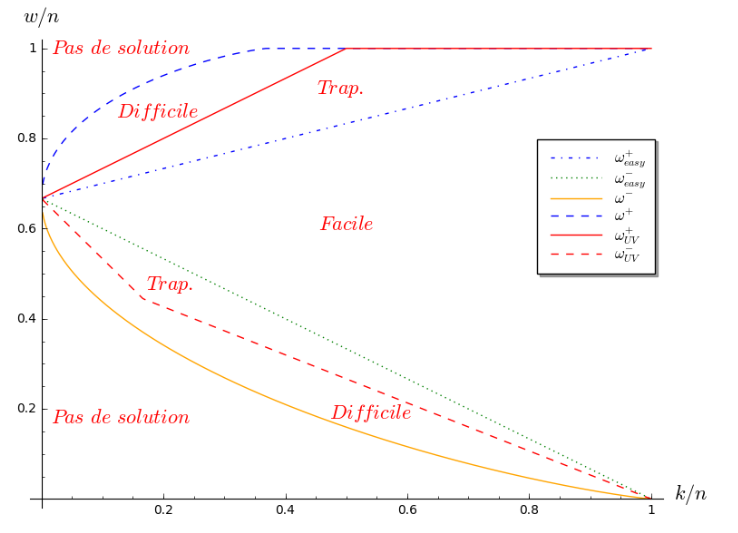
\includegraphics [scale=0.4]{include/graph_ratio_w.png}
\end{center}
\caption{\small Comparaison des distances $w/n$ avec et sans trappe en fonction du rendement.}
\label{graphique ratio}
\end{figure}

\noindent La connaissance de la trappe apporte donc bien un avantage puisqu'elle permet un décodage pour des erreurs de poids ne permettant pas de décodage générique. 

\begin{remarque} En pratique, notre système de signature comporterait une fonction de hachage. Ainsi, la fonction de signature prendrait en entrée un mot $m$ quelconque. Puis un aléa $r$ serait pris aléatoirement dans $\{0,1\}^{\lambda_0}$. Ce serait alors $s \leftarrow \verb|Hash| (m,r)$ qui serait signé. \verb|Sign| renverrait ensuite le couple $(\e,r)$. \\
La fonction \verb|Verify| prendrait en entrée $(m,(\e',r))$, récupèrerait $s \leftarrow \verb|Hash| (m,r)$ puis ferait ses vérifications. Ainsi un attaquant ne pourrait pas falsifier une signature à partir d'un vecteur $\e$ choisi aléatoirement dans $S_{\omega}$ et en récupérant $s = \e\mathbf{H}^T$. Sans la fonction de hachage, il aurait alors signé $s$.
\end{remarque}

\subsection{Implémentation et choix de paramètres}

Nous avons choisi d'implémenter le système de signature Wave en \verb|C|. 
Nous avons également fait le choix d'implémenter nous-même toutes les fonctions nécessaires à la manipulation des matrices. \\
Pour implémenter la clé privée, nous avons créé une structure contenant $\mathbf{H}_U$, $\mathbf{H}_V$, $S$, et $P$. La clé publique, quant à elle, est une simple matrice puisqu'il s'agit de $S\mathbf{H}P$ avec $\mathbf{H}$ la matrice de parité du code $(U,U+V)$-généralisé.\\
Nous avons donc écrit une fonction qui génère une paire de clé publique et privée, une fonction qui signe un message et une fonction qui vérifie la signature.
Notre fonction de signature appelle \verb|InvertAlg| qui, pour cacher la structure de $\mathbf{H}$, appelle la fonction \verb|DecodeUV| sur $\s(S^{-1})^T$ et renvoie la sortie récupérée multipliée par $P$. Nous obtenons alors bien une signature valide tout en ayant masqué les données lors des calculs.\\
Pour obtenir $\lambda$ bits de sécurité, les paramètres sont choisis de la façon suivante :
$$ n = \frac{\lambda}{0.0154} \quad \omega = 0.9261n \quad k_U = 0.07978\frac{n}{2} \quad k_V = 0.4201\frac{n}{2}$$
Nous les donnons ici sans démonstration, celle-ci peut-être trouvée dans la thèse de Thomas Debris-Alazard section 5.3.5.\\
Lors de nos tests sur le nombre de rejets effectués, nous trouvons en effet des résultats cohérents avec ce qui précède, nous avons en moyenne 1 rejet toutes les 20 signatures.\\

\section{Uniformisation des sorties}

\subsection{Une fuite d'information}
Afin de vérifier le deuxième point de la définition des fonctions GPVM, il est nécéssaire que les $\mathbf{e} \in f_{w,\mathbf{H}}^{-1}(\mathbf{s})$ ne révèlent pas d'information sur la structure du code $(U,U+V)$-généralisé utilisé. \\
Or, si la sortie $\mathbf{e_V}$ de \verb|DecodeV| n'est pas uniforme, alors des corrélations entre les coordonnées $\mathbf{e}_i$ et $\mathbf{e}_{i+n/2}$ du vecteur $\mathbf{e}$ apparaissent. \\

\noindent Par exemple, prenons le cas où $q=3$, et où pour tout $i \in \llbracket 1,n/2\rrbracket$, $a_i = c_i = d_i = 1$ et $b_i = 0$, et où \verb|DecodeV| est l'algorithme de Prange. \\
On a alors pour tout $\mathbf{e} = (\mathbf{e_U},\mathbf{e_U}+\mathbf{e_V})$
$$ |\mathbf{e_V}| = \# \; \{1  \leq i \leq n/2 \;|\; e_i \neq e_{i+n/2}\}$$

\begin{propo}
Si le vecteur $\mathbf{e_V}$ est obtenu par l'algorithme de Prange, alors il est de poids moyen $\frac{2}{3}(\frac{n}{2}-k_V)$.
\end{propo}

\noindent Alors, pour tout $i \in \llbracket1,n/2\rrbracket$, on a :
$$ \mathbb{P}(\mathbf{e}_i \neq \mathbf{e}_{i+n/2}) = \frac{2}{3(n/2)}(n/2-k_V)(1+o(1))$$

\noindent En revanche, pour les autres paires $(i,j)$, on a :
$$ \mathbb{P}(\mathbf{e}_i \neq \mathbf{e}_{j}) = \frac{4wn - 3w^2-w}{n(n-1)}$$

\noindent Ces deux probabilités n'ont donc aucune raison d'être égales. On a donc une fuite d'information. En effet, dans la pratique et afin de cacher la structure, on effectue une permutation sur les coordonnées de $\mathbf{e}$ lors de la signature. Si un attaquant récupère suffisemment de signatures, il pourra donc en analysant la fréquence des $\mathbf{e}_i \neq \mathbf{e}_j$ retrouver cette permutation. Il est donc nécéssaire pour la sécurité du schéma de s'assurer de l'uniformité des sorties de l'algorithme \verb|sign|.

\subsection{La méthode du rejet}
Afin de s'assurer un $\mathbf{e}$ uniforme dans son ensemble, nous allons :
\begin{itemize}
\item choisir $\mathbf{e}_V$ de façon à ce qu'il soit uniforme dans son ensemble 
\item mettre des conditions de rejet sur $\mathbf{e}_U$ en fonction du poids de $\mathbf{e}_V$ afin de supprimer le biais sur l'ensemble 
$$ m_1(x) := \# \; \{1  \leq i \leq n/2 \;;\; |(x_i, x_{i+n/2})| = 1\}$$
\end{itemize}
Avant d'expliciter nos algorithmes, il est nécéssaire d'introduire quelques notations et définitions. \\

\begin{nota} On notera :
\begin{itemize}
\item $\mathbf{e}^{unif}$ la variable aléatoire tirée uniformément dans l'ensemble $S_{w}$
\item $\mathbf{e}_V^{unif}$ la variable aléatoire tirée uniformément dans les mots de $\F_q^{n/2}$ 
\item $\mathbf{e}_U^{unif}$ la variable aléatoire tirée uniformément dans les mots de $\F_q^{n/2}$ conditionné au vecteur $\e_V^{unif}$
\end{itemize}
\end{nota}


\begin{defi} (uniforme en poids et $m_1$-uniforme)
\begin{itemize}
\item \verb|DecodeV| est dit uniforme en poids si ses sorties $\mathbf{e}_V$ sont telles que $\mathbb{P}(\mathbf{e}_V)$ n'est fonction que du poids de $\mathbf{e}_V$ quand $\mathbf{s}^V$ est tiré uniformément dans son ensemble.
\item \verb|DecodeU| est dit $m_1$-uniforme si ses sorties $\mathbf{e}_U$ sont telles que $\mathbb{P}(\mathbf{e}_U\; |\;  \mathbf{e}_V)$ n'est fonction que du poids de $\mathbf{e}_V$ et de $m_1(\varphi(\mathbf{e}_U,\mathbf{e}_V))$.
\end{itemize}
\end{defi}

\begin{lemme} Soit $\mathbf{e}$ la sortie de \verb|InvertAlg| avec $\mathbf{s}^U$ et $\mathbf{s}^V$ choisis uniformément dans leurs ensembles. Soit \verb|DecodeV| uniforme en poids et \verb|DecodeU| $m_1$-uniforme. Si pour tout $y$ et $z$ 
$$|\mathbf{e}_V| \sim |\mathbf{e}_V^{unif}|\quad \text{et} \quad\mathbb{P}(m_1(\mathbf{e}) = z\; |\; |\mathbf{e}_V| = y) = \mathbb{P}(m_1(\mathbf{e}^{unif}) = z\; |\; |\mathbf{e}_V^{unif}| = y)$$
Alors
$$ \mathbf{e} \sim \mathbf{e}^{unif}.$$
\end{lemme}

\begin{proof}[Preuve]\
Nous allons montrer qu'avec les hypothèses précédentes nous avons $\forall x \in S_{\omega} \quad \mathbb{P}(\e = x) = \mathbb{P}(\e^{unif} = x)$.\\
Soit $x \in S_{\omega}$ :
\begin{equation*}
\begin{split}
\mathbb{P}(\e = x) &= \mathbb{P}(\e_U = x_U, \e_V = x_V)\\[0.4cm]
&= \mathbb{P}(\e_U = x_U | \e_V = x_V)\mathbb{P}(\e_V = x_V)\\
\end{split}
\end{equation*}
Notre but étant de faire apparaître les expressions énoncées lors du lemme, nous allons exprimer ces deux probabilités en fonction de $|x_V| = y$ et de $m_1(x) = z$.
\begin{equation*}
\begin{split}
\mathbb{P}(\e_V = x_V) &= \mathbb{P}(\e_V = x_V, |\e_V| = y)\\[0.4cm]
&= \left.\mathbb{P}(\e_V = x_V \right| |\e_V| = y)\ \mathbb{P}(|\e_V| = y)\\[0.4cm]
&= \frac{\mathbb{P}(|\e_V| = y)}{n(y)}\\
\end{split}
\end{equation*}
avec $n(y) := \#\left\{ \left.\e \in \F_3^{n/2} \right| |\e| = y\right\}$.
De la même façon, nous obtenons :
{\footnotesize \begin{equation*}
\begin{split}
\mathbb{P}(\e_U = x_U |\ |\e_V| = y) &= \left.\mathbb{P}(\e_U = x_U ,\ m_1(\e) = z\ \right|\ |\e_V| = y)\\[0.4cm]
&= \left.\mathbb{P}(\e_U = x_U\ \right|\ m_1(\e) = z,\ |\e_V| = y)\mathbb{P}(m_1(\e) = z\ |\ |\e_V| = y)\\[0.4cm]
&= \frac{\mathbb{P}(m_1(\e) = z\ |\ |\e_V| = y)}{n(y,z)}\\
\end{split}
\end{equation*}}
avec $n(y,z) := \#\left\{ \left.\e \in \F_3^{n/2} \right|\  m_1(\e) = z\text{ et } |\e_V| = y \right\}$.\\

\noindent Ainsi nous obtenons
\begin{equation*}
\begin{split}
\mathbb{P}(\e = x) &= \frac{\mathbb{P}(m_1(\e) = z\ |\ |\e_V| = y)}{n(y,z)}\frac{\mathbb{P}(|\e_V| = y)}{n(y)}\\[0.4cm]
 &= \frac{\mathbb{P}(m_1(\e^{unif}) = z\ |\ |\e_V^{unif}| = y)}{n(y,z)}\frac{\mathbb{P}(|\e_V^{unif}| = y)}{n(y)}\\[0.4cm]
 &= \mathbb{P}(\e_U^{unif} = x_U | \e_V^{unif} = x_V)\mathbb{P}(\e_V^{unif} = x_V)\\[0.4cm]
 &= \mathbb{P}(\e^{unif} = x)\\
\end{split}
\end{equation*}
\end{proof}


\noindent Ainsi, pour que $\mathbf{e}$ soit uniformément distribué sur $S_\omega$, il suffit de choisir \verb|DecodeV| de façon à ce que ses sorties soient uniformes sur $\F_q^{n/2}$ puis d'ajouter une condition de rejet sur les sorties de \verb|DecodeU| de façon à ce que $m_1(\mathbf{e})$ conditionné à $|\mathbf{e}_V|$ soit distribué comme $m_1(\mathbf{e}^{unif})$ conditionné à $|\mathbf{e}_V^{unif}|$. \\
On peut alors introduire l'algorithme suivant :\\

\begin{algorithm}
	\caption{DecodeUV($\varphi, \s, \mathbf{H}_V, \mathbf{H}_U$)}
	\begin{algorithmic}[1]
   	 	\REQUIRE $\varphi$, $\s \in \F_q^{n-k}$ un syndrome, $\mathbf{H}_V \in \F_q^{(\frac{n}{2} - k_V) \times \frac{n}{2}}$, $\mathbf{H}_U \in \F_q^{(\frac{n}{2} - k_U) \times \frac{n}{2}}$
   	 	\ENSURE $\e = \varphi(e_U, e_V) \text{ avec } \e_U\mathbf{H}_U^T = \s^U \text{ et } \e_V\mathbf{H}_V^T = \s^V$
    	\STATE $\e_V \leftarrow \text {DecodeV}(\s^V,\mathbf{H}_V)$
    	\REPEAT 
    	\STATE $\e_U \leftarrow \text {DecodeU}(\varphi, \e_V, \s^U, \mathbf{H}_U)$
    	\STATE $\e \leftarrow \varphi(\e_U,\e_V)$
    	\UNTIL {$\text{rand}([0,1]) > r(m_1(\e),|\e_V|)$}
    	\RETURN $\e$
    \end{algorithmic}
\end{algorithm}\
\newpage

\noindent Avec :

\begin{equation*}
   \begin{split}
    r(s,t) &:= \frac{1}{M(t)}\frac{q^{unif}(s,t)}{q(s,t)}\\[.6cm]
    q(s,t) &:= \mathbb{P}(m_1(\mathbf{e})=s\;|\;|\mathbf{e}_V|=t)\\[.6cm]
    q^{unif}(s,t) &:= \mathbb{P}(m_1(\mathbf{e}^{unif})=s\;|\;|\mathbf{e}^{unif}_V|=t)\\[.6cm]
    M(t) &:= \max_{0 \leq s \leq t} \frac{q^{unif}(s,t)}{q(s,t)}\\[.6cm]
    \end{split}
\end{equation*}



\noindent Pour montrer que la sortie de notre algorithme \verb|DecodeUV| suit bien une distribution uniforme, énonçons le lemme suivant :

\begin{lemme}\label{rejet} Soient $X$ et $X^{unif}$ deux variables aléatoires à valeur dans un même ensemble $\mathcal{X}$ telles que :
\begin{itemize}
\item $X$ suit une distribution quelconque,
\item $X^{unif}$ suit une distribution uniforme.
\end{itemize} 
Pour tout $x \in \mathcal{X}$ on pose :
\begin{equation*}
   \begin{split}
    &r(x) := \frac{1}{M} \frac{\mathbb{P}(X^{unif}=x)}{\mathbb{P}(X=x)} \\[0.6cm]
    &M := \max_{y \in \mathcal{X}}\frac{\mathbb{P}(X^{unif}=y)}{\mathbb{P}(X=y)}\\[0.6cm]
    \end{split}
\end{equation*}
Alors la variable aléatoire $Y$ définie telle que:
\begin{enumerate}
\item On tire $x \in \mathcal{X}$ selon la distribution $X$
\item On tire $\theta$ uniformément dans l'intervalle $\llbracket 0,1 \rrbracket$,
\item Si $\;\theta \leq r(x)$, alors $Y$ prend la valeur $x$.
\item Sinon, on recommence.
\end{enumerate}
Alors la variable $Y$ suit une loi uniforme. 
\end{lemme}


\begin{proof}[Preuve] Remarquons d'abord que pour tout $x$:
$$0 \leq r(x) = \frac{1}{M}\frac{\mathbb{P}(X^{unif}=x)}{\mathbb{P}(X=x)} = \Bigg(\inf_{y \ in \mathcal{X}}\frac{\mathbb{P}(X=y)}{\mathbb{P}(X^{unif}=y)}\Bigg)\frac{\mathbb{P}(X^{unif}=x)}{\mathbb{P}(X=x)}\leq 1$$
Donc les coordonnées de $r$ sont donc bien des probabilités.\\

\noindent On remarque aussi que,
\begin{equation*}
   \begin{split}
    \mathbb{P}\;(\text{ "y soit accepté" }) &:= \mathbb{P}(\; \theta \leq r(x)\quad \text{et} \quad X=x\;) \\[0.6cm]
    &:=  \mathbb{P} (\theta \leq r(x)) \times\mathbb{P}(X=x) \\[0.6cm]
    \end{split}
\end{equation*}

\noindent De plus, la probabilité que $Y$ soit égal à $x$ est égale à la probabilité que $x$ ai été tiré et qu'il ai été accepté. 
\noindent Pour tout $x \in \mathcal{X}$, on a alors,
\begin{equation*}
   \begin{split}
    \mathbb{P}(Y=x) &:= \frac{ \mathbb{P}(\theta \leq r(x)) \times\mathbb{P}(X=x)}{\sum_{y \in \mathcal{X}} \mathbb{P}(\theta \leq r(y)) \times\mathbb{P}(X=y)} \\[0.6cm]
    &:=\frac{  r(x) \times\mathbb{P}(X=x)}{\sum_{y \in \mathcal{X}}  r(y) \times\mathbb{P}(X=y)}\qquad \Big(\text{car}\quad \mathbb{P}(\theta \leq r(x)) =  r(x)\Big)\\[0.6cm]
    &:=\frac{ \mathbb{P}(X^{unif}=x)}{M\times\sum_{y \in \mathcal{X}} 1/M \times\mathbb{P}(X^{unif}=y)}\qquad \Big(\text{car}\quad \sum_{y\in \mathcal{X}}\mathbb{P}(X^{unif}=y) = 1\Big)\\[0.6cm]
    &:= \mathbb{P}(X^{unif}=x) \\[0.6cm]
    \end{split}
\end{equation*}

\end{proof}



\noindent On peut alors énoncer la proposition suivante :


\begin{propo}
Si \verb|DecodeV| est uniforme en poids et si \verb|DecodeU| est $m_1$-uniforme, alors on a $\mathbf{e}\sim\mathbf{e}^{unif}$.
\end{propo}

\begin{proof}[Preuve]
Soit $\e_U'$ le vecteur obtenu à la sortie de la boucle dans \verb|DecodeUV|.  Notons pour tout $i,j \in \llbracket 1,n \rrbracket$:
$$q'(i,j) := \mathbb{P}(m_1(\mathbf{e'}_U)=i\;|\;|\mathbf{e'}_V|=j)$$

\noindent On a alors par le lemme \ref{rejet}
$$q'(i,j) = q^{unif}(i,j)$$
De plus la sortie de l'algorithme \verb|DecodeV| est uniforme, ce qui conclut la preuve.
\end{proof}

\subsection{Choix des algorithmes de décodage}

\noindent Nous allons maintenant détailler les algorithmes \verb|DecodeU| et \verb|DecodeV| utilisés lors de \verb|DecodeUV|. \\
Nous n'avons aucune contrainte sur la sortie de $\e_V$ si ce n'est qu'elle doit être uniforme. Nous avons donc choisi, contrairement à ce qui est spécifié dans l'article que nous avons étudié, de choisir $\e_V$ directement de façon à ce qu'il soit aléatoire. Celui est décrit ci-dessous :

\begin{algorithm}
	\caption{DecodeV($\s^V$)}
	\begin{algorithmic}[1]
    	\STATE $c$ mot aléatoire du code $V$
    	\STATE $\s \leftarrow$ le syndrome $\s^V$ paddé avec des zéros
    	\STATE $\e_V \leftarrow \s + c$
    	\RETURN $\e_V$
    \end{algorithmic}
\end{algorithm}

\noindent Nous prenons donc un mot aléatoire du code que nous ajoutons au syndrome voulu (celui-ci ayant été complété avec des zéros pour être de la bonne longueur). 
Nous obtenons alors bien une erreur choisi uniformément dans les mots à distance $\s^V$ du code.\\

\noindent En revanche, dans l'algorithme \verb|DecodeU|, nous avons des contraintes supplémentaires sur les coordonnées de $\e_U$ pour garantir un poids de $\e$ élevé. De plus, nous ajoutons le paramètre $d\in [0,k_U]$ dans le but de minimiser le nombre de rejets, en effet en fixant $k_U - d$ positions de $\e_U$, nous dépendrons moins de la structure du code et l'erreur se rapprochera donc plus de l'uniforme.

\begin{algorithm}
	\caption{DecodeU($\varphi, \e_V, \s^U, \mathbf{H}_U$)}
	\begin{algorithmic}[1]
		\STATE $t \leftarrow |\e_V|$
		\STATE $k_0 \hookleftarrow \mathcal{D}_U^t$
		\REPEAT
		\STATE $\mathcal{I} \leftarrow$ ensemble d'information de $\langle\mathbf{H}_U\rangle^\perp$
		\STATE $\mathcal{J} \subset \mathcal{I}$ de taille $k-d$ tel que $|\e_V|_\mathcal{J} = k_0$
		\STATE $x_U \hookleftarrow \{x\in\F_3^{n/2} | \forall j\in\J,  x_j \notin \{-\frac{b_i}{a_i}\e_{V_i}, -\frac{d_i}{c_i}\e_{V_i}\}\}$
		\STATE $\e_U \leftarrow \textsc{Prange }(\mathbf{H}_U, \s^U, \mathcal{I}, x_U)$
		\UNTIL {$|\varphi(\e_U,\e_V)| \neq \omega$}
		\RETURN $\e_U$
    \end{algorithmic}
\end{algorithm}

\noindent Lors de \verb|DecodeU|, nous faisons varier les ensembles $\mathcal{I}$ et $\mathcal{J}$ pour garantir un maximum de possibilité dans le choix de $\e_U$.\\
Puis nous appelons \verb|PRANGE| qui est ici une version modifié du décodage par ensemble d'information dans lequel nous choisissons $\e_U$ égal à $x_U$ sur les positions de $\mathcal{I}$. Nous répétons tout cela jusqu'à obtenir une erreur du bon poids.

\subsection{Estimation du nombre de rejet}
Nous souhaitons estimer le nombre de rejets effectués dans notre algorithme \verb|DecodeUV| utilisant les algorithmes \verb|DecodeU|, \verb|DecodeV| définis précédemment. Pour cela, introduisons la définition suivante:

\begin{defi} (Bon ensemble).
Soient $d \leq k \leq n$, $\mathbf{H}\in\F_3^{(n-k)\times n}$ et $\varepsilon \subseteq \llbracket1,n\rrbracket$ de taile $k-d$. On dit que $\varepsilon$ est un bon ensemble pour $\mathbf{H}$ si $\mathbf{H}_{\overline{\varepsilon}}$ est de rang plein. Sinon, on dit que $\varepsilon$ est un mauvais ensemble.
\end{defi}


\noindent Pour estimer ce nombre de rejets moyen, nous allons comparer $\e$ la sortie de \verb|DecodeUV| avec $\e^{unif}$ une erreur aléatoire uniforme de poids $\omega$.\\
Nous savons que la sortie de \verb|DecodeV| est uniforme, nous allons donc étudier la sortie de \verb|DecodeU|.
Nous introduisons pour cela \verb|VarDecodeU| qui fonctionne de la même façon que \verb|DecodeU| quand $\J$ est un bon ensemble pour $\mathbf{H}$ et qui renvoie une erreur aléatoire selon la distribution $\D_U^t$ sur $\J$ dans le cas contraire.
Il n'y a donc aucune raison que la sortie soit une solution du problème de décodage lorsque $\J$ n'est pas un bon ensemble pour $\mathbf{H}$.
Nous pouvons facilement voir que \verb|VarDecodeU| est $m_1$-uniforme.\\
\noindent La sortie de l'algorithme \verb|DecodeUV| utilisant \verb|VarDecodeU| est alors uniforme, on la note $\e^{unif}$.\\

\begin{defi}\
\begin{itemize}
\item $J_{x_V,l}^{unif}$ et un ensemble choisi uniformément tel que $J_{x_V,l}^{unif}\subseteq \llbracket 1,n/2 \rrbracket$, il est de cardinal $k_U-d$ et $\#J_{x_V,l}^{unif}\cap Supp(x_V) = k_0$. 
\item $J_{x_V, l}^{\mathbf{H}_U}$ est défini de la même façon avec une contrainte supplémentaire : il fait parti des bons ensembles pour $\mathbf{H}_U$.
\end{itemize}
\end{defi}

\noindent Pour plus de simplicité, nous les noterons par la suite $J^{unif}$ et $J^{\mathbf{H}_U}$.\\

\noindent Pour pouvoir compter le nombre de rejets, nous allons avoir besoin des lemmes suivants dont les preuves sont en annexes.

\begin{lemme}\label{maj_dist_e_eunif}
Nous pouvons majorer la distance statistique entre la sortie de l'algorithme utilisant \verb|DecodeU| et celle de l'algorithme utilisant \verb|VarDecodeU| de la façon suivante :
$$ \rho\left(\e ,\e^{unif}\right) \leq \sum\limits_{x_V,l} \rho\left(J^{\mathbf{H}_U},J^{unif}\right)\mathbb{P}\left(k_0 = l, \e_V = x_V\right) $$ 
\end{lemme}


\begin{lemme}\label{esp}
L'espérance de la différence statistique entre l'ensemble $J^{unif}$ choisi uniformément et l'ensemble $J^{\mathbf{H}_U}$ choisi parmi les bons ensembles pour $\mathbf{H}$ peut être majorée comme suit :
$$ \mathbb{E}\left(\rho\left(J^{unif},J^{\mathbf{H}_U}\right)\right) \leq \frac{3^{-d}}{2} $$
\end{lemme}

\begin{lemme}\label{markov}(Inégalité de Markov).\\
Soit $Z$ une variable aléatoire supposée presque sûrement positive ou nulle, alors $$\forall a>0\quad \mathbb{P}(Z > a) \leq \frac{\mathbb{E}(Z)}{a}$$
\end{lemme}

\noindent Nous pouvons maintenant énoncer le théorème suivant :

\begin{thm}\label{rejet}
Soit $\e$ la sortie de \verb|DecodeUV| et $\e^{unif}$ la variable aléatoire uniformément distribuée parmi les mots de poids $\omega$. On a :
$$ \mathbb{P}\left(\rho(\e,\e^{unif})>3^{-d/2}\right) \leq \frac{3^{-d/2}}{2} $$
\end{thm}

\begin{proof}[Preuve]
\begin{equation*}
\begin{split}
\mathbb{P}&\big(\rho(\e,\e^{unif})>3^{-d/2}\big) \\[0.4cm]
&\leq 3^{d/2}\mathbb{E}(\rho\left(\e,\e^{unif})\right) \quad \text{par l'inégalité de Markov}\\[0.4cm]
&\leq 3^{d/2}\mathbb{E}\left(\sum\limits_{x_V,l} \rho\left(J^{\mathbf{H}_U},J^{unif}\right)\mathbb{P}\left(k_0 = l , \e_V = x_V\right)\right) \text{ d'après le lemme \ref{maj_dist_e_eunif}}\\[0.4cm]
&\leq 3^{d/2}\left(\sum\limits_{x_V,l} \frac{3^{-d}}{2}\mathbb{P}\left(k_0 = l ,\e_V = x_V\right)\right) \quad \text{par \eqref{esp}}\\[0.4cm]
&= 3^{d/2} \frac{3^{-d}}{2}\left(\sum\limits_{x_V,l}\mathbb{P}\left(k_0 = l ,\e_V = x_V\right)\right) \\[0.4cm]
&= \frac{3^{-d/2}}{2}\\[0.4cm]
\end{split}
\end{equation*}
\end{proof}


\noindent La probabilité d'avoir un rejet équivaut à la probabilité d'avoir une distance significative entre $\e$ et $\e^{unif}$. D'après le théorème \ref{rejet}, nous voyons donc qu'en faisant augmenter $d$, nous serons en mesure d'effectuer très peu de rejets.


\section{Sécurité du schéma}
Pour montrer la sécurité du schéma, nous allons dans un premier temps montrer que si la matrice de parité du code considéré est difficile à distinguer d'une matrice aléatoire, alors le schéma est sûr au sens EUF-CMA.\\
Nous discuterons ensuite de la difficulté de distinguer notre matrice de parité permutée d'une matrice aléatoire. \\

\subsection{Sécurité EUF-CMA}
Nous allons montrer que le schéma est sûr au sens EUF-CMA (Existential Unforgeability under Chosen Message Attacks). Pour cela nous ferons une réduction au problème DOOM.
\subsubsection{Définitions}

Soit $\mathcal{A}$ un adversaire ayant accès à $N_{sign}$ signatures de son choix. Soit les trois algorithmes suivants :


\begin{algorithm} [h]
	\caption{Init($\lambda$)}
	\begin{algorithmic}[1]
    	\STATE $(pk,sk) \Longleftarrow$ Gen$(1^\lambda)$ 
    	\STATE $\mathbf{H}_{pk} \Longleftarrow pk$
    	\STATE $(\varphi,\mathbf{H}_{U},\mathbf{H}_{V})\Longleftarrow sk$
    	\RETURN $\mathbf{H}_{pk}$
    \end{algorithmic}
\end{algorithm}

\begin{algorithm}[h]
	\caption{Sign($s$)}
	\begin{algorithmic}[1]
    	\STATE $\e \leftarrow \mathcal{D}_{\varphi,\mathbf{H}_{U},\mathbf{H}_{V}}(\s)$
    	\RETURN $\e$
    \end{algorithmic}
\end{algorithm}

\begin{algorithm}[h]
	\caption{Fin($(s,e)$)}
	\begin{algorithmic}[1]
    	\RETURN $(\mathbf{e}\mathbf{H}_{pk}^T = s) \land (|\mathbf{e}| = \omega)$
    \end{algorithmic}
\end{algorithm}

\noindent Le jeu EUF-CMA se déroule comme suit. $\mathcal{A}$ fait appel à \verb|Init|. Il peut ensuite faire $N_{sign}$ requêtes à \verb|sign|. Le jeu est dit réussi si $\mathcal{A}$ est capable de donner $(s,e)$ accepté par \verb|Fin| et tel que $s$ n'est jamais été demandé à \verb|Sign|. \\
On définit alors le succès EUF-CMA comme :
$$Succ^{EUF-CMA}_{Wave}(t,N_{sign}) := \max_{\mathcal{A};|A|\leq t}(\mathbb{P}(\mathcal{A}\text{ réussit le jeu EUF-CMA de Wave})).$$
Le protocole est alors sûr au sens EUF-CMA si ce succès est négligeable. \\

\noindent Nous souhaitons donc montrer que notre système est sûr au sens EUF-CMA. Pour cela, nous allons dans la section suivante majorer ce succès par rapport au succès d'un problème connu, le problème DOOM.


\subsubsection{Réduction au problème DOOM}
\textbf{Le problème DOOM.} Soient des paramètres $(n,q,k,\omega,N)$, où $N$ est un entier. \\

\leftskip=1cm
\noindent \textbf{I :} $\mathbf{H}$ une matrice uniforme de $\F_q^{(n-k)\times n}$ et $(\mathbf{s}_1,...,\mathbf{s}_N)$ une liste de $N$ syndromes. 

\noindent \textbf{Q :} Décoder l'un des syndromes à la distance $w := \lfloor \omega n \rfloor$. \\

\leftskip=0cm

\noindent On définit alors le succès de DOOM comme :
$$Succ^{DOOM(n,q,k,N)}(t) := \max_{\mathcal{A};|A|\leq t}(\mathbb{P}(\mathcal{A}(\mathbf{H},\mathbf{s}_1,...,\mathbf{s}_n)=\mathbf{e}\text{ tel que }$$
$$ \mathbf{eH}^T = \mathbf{s}_j \text{ pour un certain } j \in \{1,...,N\})).$$

\noindent La réduction à ce problème est naturelle pour un schéma de signature. Il suffit de s'assurer que l'on peut considérer notre matrice de parité comme une matrice d'un code aléatoire. Ainsi, si $\mathcal{A}$ arrive à créer une signature valide sans connaître l'algorithme de décodage $\mathcal{D}_{\varphi,\mathbf{H}_{U},\mathbf{H}_{V}}$, il a bien résolu le problème du décodage. Puisqu'on a montré préalablement que les sorties $\e$ de \verb|sign| sont uniformément distribuées sur $S_{\omega}$, la connaissance des $N_{sign}$ couples $(\s,\e)$ ne donnent pas d'avantage à $\mathcal{A}$. Ainsi la réduction se fait naturellement. \\


\subsubsection{Preuve formelle de la réduction}
Afin de faire une preuve formelle de la sécurité EUF-CMA, nous allons changer le jeu en rajoutant une fonction de hachage. L'attaquant $\mathcal{A}$ peut maintenant faire $N_{hash}$ appelle à la fonction de hachage et ainsi obtenir des couples (m,s). Il cherchera alors à créer une signature valide pour l'un d'entre eux. On retrouve bien la question du problème DOOM. \\
De plus, la fonction de signature prends maintenant en entrée un message quelconque. Elle prend ensuite un aléa $r$ dans $\{0,1\}^{\lambda_0}$. Le tout est alors donné à la fonction de hachage qui renvoit un syndrome valide. \\

\noindent Nous allons aussi introduire un système de jeux qui nous permettra de réduire la sécurité d'un système à un problème $P$. Soit $\mathcal{A}$ un attaquant et $\mathcal{R}$ un rival. Soient $G_0, G_1, ...,G_N$ un ensemble de jeux et soit $\mathbb{P}(G_i)$ la probabilité pour $\mathcal{A}$ de répondre au défi posé par $\mathcal{R}$ pour le jeu $G_i$. $\mathbb{P}(G_0)$ est alors la probabilité de cassé le système considérer et $\mathbb{P}(G_N)$ la probabilité de répondre au problème $P$. \\
L'idée est de changer pas à pas les jeux $G_0$ à $G_N$ de façon à ce que :
$$\forall i \in {0,...,N-1}, |\mathbb{P}(G_i)-\mathbb{P}(G_i+1)| \in negl(\lambda) \Longrightarrow |\mathbb{P}(G_0)-\mathbb{P}(G_N)|  \in negl(\lambda)$$
où $\lambda$ est un paramètre de sécurité. Autrement dis, les changements sur les jeux ne changent qu'à un facteur négligeable près les probabilités de succès de l'attaquant $\mathcal{A}$. \\
Il n'est pas possible de changer le comportement de $\mathcal{A}$ puisqu'il est quelconque, en revanche nous pouvons modifier celui de $R$. \\

\begin{thm} (Réduction de sécurité).\label{DOOM} \\
Soit $N_{sign}$ le nombre de requêtes faites à l'oracle de signature. Soit $\lambda$ le paramètre de sécurité et $\lambda_0=\lambda + 2\log_2(N_{sign})$. On a :
$$Succ^{EUF-CMA}_{Wave}(t,N_{sign}) \leq 2Succ^{DOOM(n,q,k,N)}(t) +\rho(\mathcal{D}_{rand},\mathcal{D}_{pub})(t) + $$
$$ f(\mathcal{U}_{\omega},\mathcal{D}_{\omega}^{\mathbf{H}_{pk}}) + g(\epsilon) + c + \frac{N_{hash}}{2}\sqrt{\epsilon} + \frac{1}{2^{\lambda}}$$
où $\epsilon$ est une fonction en $n$ qui décroît exponentiellement, $\mathcal{D}_{rand}$ est la distribution des matrices prises aléatoirement dans $\F_q{(n-k)\times n}$, $\mathcal{D}_{pub}$ celle des matrices prises aléatoirement dans l'ensemble des matrices de parité d'un code $(U,U+V)$-généralisé (et $U$, $V$ de dimension respectives $k_U$ et $k_V$), $f$ l'espérance de la distance calculatoire entre les deux distributions, $g$ linéaire en $\epsilon$ et $c$ une constante.
\end{thm}

\begin{proof}[Preuve] (On trouvera le détail des preuves de probabilité en annexe de ce rapport.) On rappelle que $G_0$ correspond à notre jeu pour la sécurité EUF-CMA de Wave.
\begin{itemize} 
\item $G_1$ : Le jeu $G_1$ est identique au jeu $G_0$ sauf si l'évènement 
\begin{center}
$F := \{\text{Un même aléa r a été tiré lors de deux requêtes}$
$\text{\qquad d'un même message à l'oracle de signature}\}.$
\end{center}
On a alors 
$$ \mathbb{P}(G_0) \leq  \mathbb{P}(G_1) +  \mathbb{P}(F) $$
Or pour $\lambda_0=\lambda + 2\log_2(N_{sign})$, la probabilité que l'évènement $F$ se produise est majorée par $\frac{1}{2^{\lambda}}$. C'est donc négligeable et le changement est autorisé.
\item $G_2$ : Le passage au jeu $G_2$ permet d'empêcher $\A$ de faire appel à l'oracle de signature sur les syndrome du problème DOOM. L'idée est de créer une liste suffisemment grande $L_m$ d'aléas tous différents. On modifie alors la fonction \verb|hash| de cette façon :
	\begin{enumerate}
	\item Si \verb|hash| est appelée par la fonction \verb|sign|, alors les aléas seront pris successivement dans $L_m$ et associés à un vecteur erreur $\e_{m,r}$ (stocké) pris uniformément dans $S_{\omega}$. Elle renvoie alors $\s=\e_{m,r}\mathbf{H}^T$.
	\item En revanche si \verb|hash| est appelée hors de la fonction \verb|sign| par $\A$, alors elle son comportement dépendra de l'aléa. Si $r$ est dans $L_m$ elle se comporte comme si elle avait été appelée par \verb|sign| et renvoie $\e_{m,r}\mathbf{H}^T$. Sinon elle renvoie successivement les syndromes du problème DOOM.
	\end{enumerate}
On prend donc dans la fonction \verb|sign| toujours le $r$ suivant de $L_m$. On a alors changé le jeu en supprimant le cas où deux mêmes $r$ sont tirés lors de la signature. Cela ne pose pas de problème grace au passage à $G_1$. Le passage au jeu $G_2$ permettra ainsi de s'assurer par la suite que $\A$ n'a pas fait d'appel à \verb|sign| sur les syndromes du problème DOOM.
On a alors 
$$ \mathbb{P}(G_1) \leq  \mathbb{P}(G_2) +  \frac{N_{hash}}{2}\sqrt{\epsilon} $$
où $\epsilon$ est une fonction en $n$ qui décroît exponentiellement. C'est donc bien négligeable.
\item $G_3$ : Le jeu $G_3$ permet à l'oracle de signature de se passer de l'algorithme de décodage, et donc de la trappe $T$. Il sera nécessaire pour remplacer la matrice du code (U,U+V)-généralisé par la matrice aléatoire de l'instance du problème DOOM. Pour passer au jeu $G_3$, on modifie la sortie de \verb|sign|. Au lieu de renvoyer le couple $(\e,r)$ où $\e = D_{\varphi,H_U,H_V}$, on renvoit le couple $(\e_{m,r},r)$ préalablement stocké.\\
 La différence de succès de dépand que de $\omega$ et des différence de distribution entre $\mathcal{U}_{\omega}$ et $\mathcal{D}_{\omega}^{\mathbf{H}_{pk}}$, où $\mathcal{U}_{\omega}$ et la distribution uniforme sur $S_{\omega}$ et où $\mathcal{U}_{\omega}$ et $\mathcal{D}_{\omega}^{\mathbf{H}_{pk}}$ est la distribution des couples $(e,r)$ où $r$ est un aléa uniforme dans $\{0,1\}^{\lambda_0}$ et $e$ est la sortie de l'algorothme de décodage avec trappe sur une entrée $s$ prise uniformément dans $\F_q^{n-k}$.
On a alors 
$$ \mathbb{P}(G_2) \leq  \mathbb{P}(G_3) + f(\mathcal{U}_{\omega},\mathcal{D}_{\omega}^{\mathbf{H}_{pk}}) + g(\epsilon) + c$$
où $f$ et $g$ sont linéaires et $c$ un certaine constante.
\item $G_4$ : On peut maintenant remplacer $\mathbf{H}_{pk}$ par $\mathbf{H}_0$. Ce changement ne pose pas de problème puisque \verb|sign| n'utilise plus la trappe. En revanche, nous avons créé un distingueur entre la distribution $(:=\mathcal{D}_{rand})$ des matrices prises aléatoirement dans $\F_q{(n-k)\times n}$ et la distribuction $(:=\mathcal{D}_{pub})$ des matrices prises aléatoirement dans l'ensemble des matrices de parité d'un code $(U,U+V)$-généralisé où $U$ (resp. $V$) est un $[n/2,k_U]$-code (resp. $[n/2,k_V]$-code). 
On a alors 
$$ \mathbb{P}(G_3) \leq  \mathbb{P}(G_4) + \rho(\mathcal{D}_{rand},\mathcal{D}_{pub})(t)$$
\item $G_5$ : On change ici la procédure de fin. On rajoute à la vérification la condition $r \notin L_m$. Ainsi on est bien sûr que $\A$ réussi le jeu s'il répond au problème DOOM. Alors la probabilité que $\A$ réussisse $G_5$ est exactement la probabilité que $\A$ réussisse $G_4$ et $r\notin L_m$.
On a alors 
$$ \mathbb{P}(G_4) \leq  2\mathbb{P}(G_5) + \rho(\mathcal{D}_{rand},\mathcal{D}_{pub})(t)$$
où $\mathbb{P}(G_5)$ est exactement la probabilité pour $\A$ de renvoyer $\e_j \in S_{\omega}$ et tel que $\e_j\mathbf{H}_0^T = \s_j$ pour un certain indice $j$ du problème DOOM. On a donc 
$$ \mathbb{P}(G_5) \leq Succ^{n,k,N_{hash}, \omega}_{DOOM}(t)$$
\end{itemize}
En rassemblant toutes les inégalités on termine la preuve. 
\end{proof}


\subsection{Indistinguabilité des codes (U,U+V)-généralisés}
Le schéma Wave est, d'après ce qui précède, sûr à condition que l'on ne puisse pas distinguer une matrice de parité d'un code (U,U+V)-généralisé d'une matrice de parité aléatoire. \\

\noindent Nous avons, tout au long de ce rapport, simplifié les notations et les algorithmes. Afin de discuter ce problème de distinction, il est nécéssaire d'en réintroduire certaines. \\
La trappe du schéma Wave étant la structure du code $(U,U+V)$-généralisé utilisé, nous devons nous assurer qu'on ne peut pas la retrouver à partir de la clé secrète. Nous introduisons donc une matrice $S\in\F_q^{(n-k)\times(n-k)}$ inversible et une matrice de permutation $P\in\F_q^{n\times n}$, la clé publique devient alors $pk = SHP$. Les matrices $S$ et $P$ faisant donc partie de la clé privée. Ainsi, on peut espérer que la matrice de parité de laisse plus apparaître cette structure. \\

\noindent Lorsque $\dim(U) < \dim(V)$, il est possible de montrer que ce problème est NP-complet à l'aide d'une réduction au problème du mariage tri-dimensionnel lui-même NP-complet. \\
Malheureusement notre algorithme de décodage ne fonctionne pas dans le cas où $\dim(U) < \dim(V)$. En effet, afin d'obtenir des erreurs de grands poids et d'assurer qu'il sera difficile de décoder sans trappe, on a fixé $2k_U$ coordonnées de $e$. Si $\dim(U) < \dim(V)$, alors le fait que $e$ soit de poids supérieur ou égal à $2k_U$ ne suffit plus à sortir de l'intervalle $\llbracket \omega^-_{easy},\omega^+_{easy}\rrbracket$. \\

Nous devons donc nécéssairement nous placer dans où $\dim(U) > \dim(V)$. Or nous avons montré précédemment qu'il est alors facile de distinguer un code binaire $(U,U+V)$-généralisé d'un code aléatoire. On fixe alors $q>2$. \\
La démonstration du caractère NP-complet de Wave lorsque $q=3$ et $\dim(U) > \dim(V)$ reste non achevée pour l'instant.
Les auteurs du papier pensent néanmoins que la généralisation des codes $(U,U+V)$ comme nous l'avons présentée dans la définition \ref{UV-normalise} et notamment le grand choix des vecteurs $a$, $b$, $c$, et $d$ offrent la possibilité d'étendre la réduction au problème du mariage tri-dimensionnel.\\

\newpage
\section*{Conclusion}
\addcontentsline{toc}{section}{\protect\numberline{}Conclusion}
Le schéma de signature Wave présente une solution originale pour répondre aux problèmes rendant difficile la génération de signatures à base de codes correcteurs. Il est le premier, et actuellement seul, cryptosystème utilisant des codes avec un décodage en grande distance.
La méthode du rejet, ajoutée afin de garantir des signatures uniformément distribuées, empêche bien toute fuite d'information sur la structure du code à partir de la signature $e$. De plus, c'est une solution très efficace, puisque le nombre de rejet effectués est surprenamment faible. \\
Dans notre implémentation, nous avons effectivement constaté un très petit nombre de rejets. \\
En revanche, il y a encore peu de certitudes sur l'indistinguabilité des matrices de parités, ce qui remet en question les preuves de sécurité. On peut cependant espérer que la grande liberté sur le choix des vecteurs $a,b,c,d$ permettrait une réduction de sécurité dans les cas qui nous intéressent. 


\newpage

\begin{appendix}
\section*{Quelques preuves supplémentaires}
\addcontentsline{toc}{section}{\protect\numberline{}Quelques démonstrations supplémentaires}

\subsection*{Démonstration du lemme \ref{maj_dist_e_eunif}}

Nous allons avoir besoin dans la suite de la proposition suivante que nous ne démontrerons pas dans ce rapport :
\begin{propo}\label{rho_f}
Soient $X$ et $Y$ deux variables aléatoires dans le même espace $A$ et $Z$ une variable aléatoire dans l'espace $B$ indépendante de $X$ et $Y$. Alors, pour toute fonction $f$, nous avons : $$ \rho(f(X,Z),f(Y,Z)) \leq \rho(X,Y)$$
\end{propo}

\begin{proof}[Preuve du lemme \ref{maj_dist_e_eunif}]
Rappelons que nous voulons montrer l’inégalité :
$$ \rho\left(\e ,\e^{unif}\right) \leq \sum\limits_{x_V,l} \rho\left(J^{\mathbf{H}_U},J^{unif}\right)\mathbb{P}\left(k_0 = l, \e_V = x_V\right) $$ 

\noindent En écrivant $\e = (\e_U,\ \e_V)$ et $\e^{unif} = (\e_U^{unif},\ \e_V^{unif})$, nous pouvons majorer leur distance statistique
{\scriptsize
\begin{equation*}
\begin{split}
\rho(\e,\e^{unif}) &= \rho\Big((\e_U,\e_V),(\e_U^{unif},\e_V^{unif})\Big)\\
&\leq \sum\limits_{x_U,x_V} \left|\mathbb{P}\Big((\e_U,\e_V)=(x_U,x_V)\Big) - \mathbb{P}\Big((\e_U^{unif},\e_V^{unif})=(x_U,x_V)\Big)\right|\\
&= \sum\limits_{x_U,x_V} \left|\mathbb{P}(\e_V = x_V)\mathbb{P}(\e_U=x_U|\e_V=x_V) - \mathbb{P}(\e_V^{unif} = x_V)\mathbb{P}(\e_U^{unif}=x_U | \e_V^{unif}=x_V)\right|\\
&= \sum\limits_{x_U,x_V} \mathbb{P}(\e_V = x_V)\left|\mathbb{P}(\e_U=x_U|\e_V=x_V) - \mathbb{P}(\e_U^{unif}=x_U | \e_V^{unif}=x_V)\right|\\
\end{split}
\end{equation*}}

\noindent Le passage de la troisième ligne à la quatrième se fait car $\mathbb{P}(\e_V = x_V) = \mathbb{P}(\e_V^{unif} = x_V) $.

\noindent Rappelons que $k_0$ est le poids de $\e_V$ sur $J$, en ajoutant une condition sur la valeur de $k_0$ aux probabilités, nous obtenons donc la somme suivante :
{\scriptsize
$$ \mathbb{P}(\e_U=x_U|\e_V=x_V) - \mathbb{P}(\e_U^{unif}=x_U | \e_V^{unif}=x_V) =  $$
$$ \sum\limits_l \left[ \mathbb{P}(\e_U=x_U|k_0 = l,\e_V=x_V) - \mathbb{P}(\e_U^{unif}=x_U |k_0 = l, \e_V^{unif}=x_V) \right] \mathbb{P}\left(k_0 = l | \e_V =x_V\right)$$
}

\noindent Nous obtenons donc, comme majoration de la distance statistique, une somme sur les indices $x_U$, $x_V$ et $l$. Nous allons maintenant étudier la somme sur les indices $x_U$.\\
\noindent Les ensembles $\J$ étant inclus dans un ensemble d'information, l'aléa interne de \verb|DecodeU| et de \verb|VarDecodeU| ne dépendent pas du choix de $J^{unif}$ et $J^{\mathbf{H}_U}$. 
Nous pouvons voir que $\mathbb{P}(\e_U=x_U|k_0 = l,\e_V=x_V)$ ne dépend que de $x_U$ et $J^{\mathbf{H}_U}$ et   $\mathbb{P}(\e_U^{unif}=x_U |k_0 = l, \e_V^{unif}=x_V)$ ne dépend que de $x_U$ et $J^{unif}$. 
De plus, $J^{unif}$ et $J^{\mathbf{H}_U}$ vivent dans le même espace.
Ainsi d'après la proposition \ref{rho_f}, nous avons 
{\scriptsize
$$ \sum\limits_{x_U}\mathbb{P}(\e_U=x_U|k_0 = l,\e_V=x_V) - \mathbb{P}(\e_U^{unif}=x_U |k_0 = l, \e_V^{unif}=x_V)\quad \leq\quad \rho(J^{\mathbf{H}_U},J^{unif})$$
}

En combinant les différentes équations obtenues, nous avons alors :
\begin{equation*}
\begin{split}
\rho\left(\e ,\e^{unif}\right) &\leq \sum\limits_{x_V,l} \rho\left(J^{\mathbf{H}_U},J^{unif}\right)\mathbb{P}(\e_V = x_V)\mathbb{P}\left(k_0 = l| \e_V = x_V\right)\\
&=\sum\limits_{x_V,l} \rho\left(J^{\mathbf{H}_U},J^{unif}\right)\mathbb{P}\left(k_0 = l, \e_V = x_V\right)
\end{split}
\end{equation*}
\end{proof}

\subsection*{Démonstration du lemme \ref{esp}}

\begin{lemme}\label{proba_rang}
Soient $d$ et $m$ deux entiers tels que $d<m$ et $M \hookleftarrow\F_3^{(m-d)\times m}$ alors $\mathbb{P}(rg(M) < m-d) \leq \frac{1}{2 . 3^d}$
\end{lemme}

\begin{proof}[Preuve]
Soit $P$ la probabilité que $M$ ne soit pas de rang plein, c'est-à-dire de rang inférieur à $m-d$.
Notons $V_i$ le sous-espace vectoriel engendré par les $i$ premières lignes de $M$. Si $M$ n'est pas de rang plein c'est qu'au moins une de ses lignes est une combinaison linéaire des précédentes, c'est-à-dire qu'il existe un $i$ tel que $\dim(V_i) = \dim(V_{i-1}) = i-1$. On a alors
\begin{equation*}
\begin{split}
P &\leq \sum\limits_{i=1}^{m-d} \mathbb{P}(\dim(V_i) = \dim(V_{i-1}) = i-1) \\
&= \sum\limits_{i=1}^{m-d} \mathbb{P}(\dim(V_i) =i-1 | \dim(V_{i-1}) = i-1)\mathbb{P}(\dim(V_{i-1}) = i-1) \\
&\leq \sum\limits_{i=1}^{m-d} \mathbb{P}(\dim(V_i) =i-1 | \dim(V_{i-1}) = i-1) \\
\end{split}
\end{equation*}
Si $\dim(V_{i-1}) = i-1$, alors $\dim(V_i) = i-1$ est équivalent à dire que la ligne $i$ de la matrice est une combinaison linéaire des $i-1$ précédentes. Nous avons donc :
$$ \mathbb{P}(\dim(V_i) =i-1 | \dim(V_{i-1}) = i-1) = \frac{3^{i-1}}{3^m} = \frac{1}{3^{m-i+1}} $$
Nous pouvons donc conclure avec :
\begin{equation*}
\begin{split}
P &\leq \sum\limits_{i=1}^{m-d} \frac{1}{3^{m-i+1}}\\
& = \frac{1}{2.3^{-d}} - \frac{1}{2;3^m}\\
&\leq  \frac{1}{2.3^{-d}} 
\end{split}
\end{equation*}
\end{proof}

\begin{proof}[Preuve du lemme \ref{esp}]

Nous voulons ici montrer que $$ \mathbb{E}\left(\rho\left(J_{x_V,l}^{unif},J_{x_V, l}^{\mathbf{H}_U}\right)\right) \leq \frac{3^{-d}}{2} $$
Notons $n_{U,d}$ le nombre de sous-ensembles de $\llbracket 1, n/2\rrbracket$ de taille $k_U-d$ ie \mbox{$n_{U,d} = $ {\scriptsize$\dbinom{n/2}{k_U-d}$}}. On a alors $$\rho(J^{unif},\ J^{\mathbf{H}_U}) = \frac{N}{n_{U,d}}$$ avec $N = \#\{J \subset \llbracket 1,\ n/2\rrbracket \text{ de taille } k_U - d \text{ mauvais pour } \mathbf{H}_U\}$.\\
Notons $X_i$ l'événement "le sous-ensemble $\varepsilon_i$ est un mauvais ensemble pour $\mathbf{H}_U$", c'est-à-dire la matrice $M_{\overline{\varepsilon_i}}$ n'est pas de rang plein. D'après le lemme \ref{proba_rang}, nous avons $\mathbb{P}(X_i = 1)\leq \frac{1}{2.3^d}$
De plus, nous pouvons maintenant écrire $N = \sum\limits_{i=1}^{n_{U,d}}X_i$.\\
Ainsi nous avons :
\begin{equation*}
\begin{split}
\mathbb{E}\left(\rho\left(J_{x_V,l}^{unif},J_{x_V, l}^{\mathbf{H}_U}\right)\right)  &= \mathbb{E}\left(\frac{N}{n_{U,d}}\right)  \\
&= \mathbb{E}\Bigg(\frac{\sum\limits_{i=1}^{n_{U,d}}X_i}{n_{U,d}}\Bigg)\\
&= \sum\limits_{i=1}^{n_{U,d}}\mathbb{E}\left(\frac{X_i}{n_{U,d}}\right)\\
&= \sum\limits_{i=1}^{n_{U,d}}\frac{\mathbb{P}(X_i = 1)}{n_{U,d}}\\
&\leq \frac{1}{2.3^d}\\
\end{split}
\end{equation*}
\end{proof}


\subsection*{Démonstration du théorème \ref{DOOM}}
\begin{proof}[Preuve] \
\begin{itemize}
\item \textbf{Passage de $G_0$ à $G_1$ : } Montrons que $$\mathbb{P}(F) \leq \frac{1}{2^\lambda}$$.
Remarquons d'abord que la probabilité de n'avoir aucune collision sur $t$ tirages indépendants et uniforme dans un ensemble de taille $n$ est majoré par $t^2/n$ (admis). Dans notre cas, $t=N_{sign}$ et $n=2^{\lambda_0}$. Ainsi avec $\lambda_0 = \lambda +2 \log_2N_{sign}$, on en déduit que 
$$ \mathbb{P}(F) \leq \frac{N^2_{sign}}{2^{\lambda_0}}=\frac{1}{2^{\lambda_0 -2 \log_2N_{sign}}} =\frac{1}{2^\lambda}$$ ce qui conclu la preuve.
\item \textbf{Passage de $G_1$ à $G_2$ : } Montrons que $$ \mathbb{P}(G_1) \leq  \mathbb{P}(G_2) +  \frac{N_{hash}}{2}\sqrt{\epsilon} $$
où $\epsilon$ est une fonction en $n$ qui décroît exponentiellement.
Nous utiliserons la proposition suivante (admise) :
\begin{propo} Soient les variables aléatoires discrètes $X_i$ et $Y_i$ où $i \in \{1,2\}$ de même domaine $\mathcal{A}_i$. Notons pour $a_i \in \mathcal{A}_i$ :
	\begin{itemize}
	\item $p(.|a_i)$ la distribution de $X_2$ conditionnée à l'évènement $X_1 = a_i$
	\item $q(.|a_i)$ la distribution de $Y_2$ conditionnée à l'évènement $Y_1 = a_i$
	\end{itemize}
Alors nous avons,
$$\rho(X_1,X_2,Y_1,Y_2) \leq \sup_{a_i \in \mathcal{A}_i}\rho(p(.|a_i),q(.|a_i)) + \rho(X_1,Y_1).$$
\end{propo}
Les distributions des jeux $G_1$ et $G_2$ diffèrent par les sorties de la fonction de hachage. Dans le jeu $G_1$ les sorties $X_i$ sont uniformément distribuées dans $\F_q^{n-k}$. Dans le jeu  $G_2$, les sorties $Y_i$ valent $\e\mathbf{H}^T$ avec $e$ uniformément distribué dans $S_{\omega}$ si $r\in L_m$, sinon $Y_i$ est uniformément distribuée.  On a,
\begin{equation}
\begin{split}
\mathbb{P}(G_1) - \mathbb{P}(G_2) &= \sum_{\mathbf{H}}\mathbb{P}(\mathbf{H}_{pk}=\mathbf{H})(\mathbb{P}(G_1|\mathbf{H}_{pk}=\mathbf{H})-\mathbb{P}(G_1|\mathbf{H}_{pk}=\mathbf{H}) \\
&\leq \mathbb{E}_{\mathbf{H}_{pk}}(\rho(X_1,...,X_{N_{hash}},Y_1,...,Y_{N_{hash}}))\\
\end{split}
\end{equation}
\begin{propo} Soit $X$ la distribution uniforme dans $\F_q^{n-k}$ et $Y$ la distribution de $\e\mathbf{H}^T$ avec $e$ uniformément distribué dans $S_{\omega}$. Alors
$$\mathbb{E}_{H_{pk}}(\rho(X,Y)) \leq \frac{1}{2}\sqrt{\epsilon} $$
où $\epsilon$ est une borne qui décroit exponentiellement avec $n$.
\end{propo}
Par les deux propositions précédentes et par un raisonnement par récurrence, on termine la preuve. 
\item \textbf{Passage de $G_2$ à $G_3$ : } Nous avons
$$ \mathbb{P}(G_2) \leq  \mathbb{P}(G_3) + f(\mathcal{U}_{\omega},\mathcal{D}_{\omega}^{\mathbf{H}_{pk}}) + g(\epsilon) + c$$
où $f$ et $g$ sont linéaires et $c$ un certaine constante.
La fonction en $\epsilon$ découle d'un raisonnement similaire au raisonnement précédent. Ensuite, à constante près, les différences de distributions entre les jeux $G_2$ et $G_3$ ne dépendent que de l'espérance de la distance statistique entre les distributions $\mathcal{U}_{\omega}$ et $\mathcal{D}_{\omega}^{\mathbf{H}_{pk}}$, où $\mathcal{U}_{\omega}$ et la distribution uniforme sur $S_{\omega}$ et où $\mathcal{U}_{\omega}$ et $\mathcal{D}_{\omega}^{\mathbf{H}_{pk}}$ est la distribution des couples $(e,r)$ où $r$ est un aléa uniforme dans $\{0,1\}^{\lambda_0}$ et $e$ est la sortie de l'algorothme de décodage avec trappe sur une entrée $s$ prise uniformément dans $\F_q^{n-k}$.
\item \textbf{Passage de $G_3$ à $G_4$ : } La différence entre ces deux jeux ne vient que de la distance entre la distributions des matrices de parité de nos codes $(U,U+V)$-généralisés et celle des matrices prises uniformément dans $\F_q^{n-k}$.
\item \textbf{Passage de $G_4$ à $G_5$ : } Le jeu $G_5$ diffère du jeu $G_4$ uniquement par la vérification finale. Soit le couple $(e,r)$ la réponse de $\mathcal{A}$ comme signature d'un message $m$. Sa probabilité de succès pour le jeu $G_5$ est exatement la probabilité de l'évènement "réussit $G_4$ et $r\notin L_m$".  \\
Si la signature est valise, alors $m$ n'a jamais été demandé à l'oracle de signature, donc $\mathcal{A}$ n'a jamais eu accès aux éléments de $L_m$. Donc les évenements sont indépendants et nous avons,
$$\mathbb{P}(G_5) = (1 - 2^{- \lambda_0})^{N_{sign}}\mathbb{P}(G_4).$$
où $\lambda_0 \leq \log_2(N²_{sign})$. Donc
$$(1-2^{-\lambda_0})^{N_{sign}} \geq (1-\frac{1}{N²_{sign}})^{N_{sign}} \geq \frac{1}{2} $$

D'où $\mathbb{P}(G_5) \geq\frac{1}{2}\mathbb{P}(G_4)$.
\end{itemize}

\end{proof}


\end{appendix}

\newpage
\nocite{ref1}
\nocite{ref2}
\bibliographystyle{plain}
\bibliography{bibliography}


\end{document}
